% assembly.tex — Part 2 of the build: putting it together, in order, with a check after every stage.
% Build:  python3 tools/make_figures.py && latexmk -lualatex assembly.tex
\documentclass[10pt]{article}
\newcommand{\doctitle}{Radar build, part 2: assembly and bring-up}
% common.tex — shared preamble for the two build documents.
% Compile with LuaLaTeX (fontspec + DejaVu, so Ω µ ° × → print as themselves).
\usepackage[letterpaper,margin=19mm,top=22mm,bottom=20mm,headsep=6mm]{geometry}
\usepackage{fontspec}
\setmainfont{DejaVu Sans}[Scale=0.92]
\setsansfont{DejaVu Sans}[Scale=0.92]
\setmonofont{DejaVu Sans Mono}[Scale=0.86]
\renewcommand{\familydefault}{\sfdefault}
\usepackage{microtype}
\usepackage[table]{xcolor}
\usepackage{graphicx}
\usepackage{tikz}
\usetikzlibrary{arrows.meta,calc,positioning,patterns,decorations.pathreplacing,shapes.geometric,fit,backgrounds}
\usepackage[american,siunitx]{circuitikz}
\usepackage{booktabs,tabularx,longtable,array,multirow,makecell}
\usepackage{enumitem}
\usepackage{titlesec}
\usepackage{fancyhdr}
\usepackage{caption}
\usepackage{pdflscape}
\usepackage[most]{tcolorbox}
\usepackage[hidelinks]{hyperref}
\usepackage{float}

% ── palette (matches the horn build guide and the HFSS guide)
\definecolor{ink}{HTML}{14181D}
\definecolor{muted}{HTML}{5F6670}
\definecolor{rule}{HTML}{C9CDD3}
\definecolor{faint}{HTML}{E3E6EA}
\definecolor{accent}{HTML}{8A3B1E}
\definecolor{boxbg}{HTML}{F4EFE6}
\definecolor{cuout}{HTML}{E2A27A}
\definecolor{cuin}{HTML}{B86F45}
\definecolor{cuedge}{HTML}{6B3A1F}
\definecolor{tabfill}{HTML}{F3D2BC}
\definecolor{bend}{HTML}{1F5F8B}
\definecolor{dimc}{HTML}{3B4450}
\definecolor{wood}{HTML}{D9B98C}
\definecolor{woodedge}{HTML}{8C6A3F}
\definecolor{alu}{HTML}{B8C0C8}
\definecolor{rfmod}{HTML}{CFE0EE}
\definecolor{pcb}{HTML}{CFE3CF}
\definecolor{sig}{HTML}{2E7D32}
\definecolor{pwr}{HTML}{C62828}
\definecolor{logic}{HTML}{1565C0}
\definecolor{okgreen}{HTML}{2E7D32}
\definecolor{warnamber}{HTML}{B26A00}
\color{ink}

% ── headings
\titleformat{\section}{\Large\bfseries\color{ink}}{\color{accent}\thesection}{0.7em}{}
\titleformat{\subsection}{\large\bfseries\color{accent}}{\thesubsection}{0.6em}{}
\titleformat{\subsubsection}{\normalsize\bfseries\color{ink}}{}{0em}{}
\titlespacing*{\section}{0pt}{2pt}{8pt}
\titlespacing*{\subsection}{0pt}{12pt}{4pt}
\titlespacing*{\subsubsection}{0pt}{8pt}{2pt}
\setlength{\parindent}{0pt}
\setlength{\parskip}{5pt}
\linespread{1.08}
\setlist{itemsep=2pt,topsep=3pt,leftmargin=16pt}
\captionsetup{font={small,color=muted},labelfont={bf,color=muted},justification=raggedright,singlelinecheck=false,skip=4pt}

% ── tables
\renewcommand{\arraystretch}{1.25}
\arrayrulecolor{rule}
\newcolumntype{L}{>{\raggedright\arraybackslash}X}
\newcolumntype{P}[1]{>{\raggedright\arraybackslash}p{#1}}

% ── callouts
\newtcolorbox{note}[1][]{enhanced,colback=boxbg,colframe=boxbg,borderline west={2.4pt}{0pt}{accent},
  arc=0pt,left=8pt,right=8pt,top=4pt,bottom=4pt,fonttitle=\bfseries,coltitle=ink,
  title={#1},attach title to upper={\par\smallskip},before skip=6pt,after skip=8pt}
\newtcolorbox{warn}[1][]{enhanced,colback=warnamber!8,colframe=warnamber!8,borderline west={2.4pt}{0pt}{warnamber},
  arc=0pt,left=8pt,right=8pt,top=4pt,bottom=4pt,fonttitle=\bfseries,coltitle=warnamber!80!black,
  title={#1},attach title to upper={\par\smallskip},before skip=6pt,after skip=8pt}
\newtcolorbox{okbox}{enhanced,colback=okgreen!7,colframe=okgreen!7,borderline west={2.4pt}{0pt}{okgreen},
  arc=0pt,left=8pt,right=8pt,top=4pt,bottom=4pt,before skip=4pt,after skip=8pt}
\newcommand{\checkline}[1]{\begin{okbox}\textbf{\color{okgreen!70!black}Check.}\ #1\end{okbox}}

% ── a numbered step banner
\newcounter{stepno}
\newcommand{\step}[1]{\stepcounter{stepno}\par\smallskip
  \noindent\begin{tikzpicture}[baseline=(t.base)]
    \node[fill=accent,text=white,font=\bfseries,minimum width=7mm,minimum height=6mm,inner sep=2pt](n){\thestepno};
    \node[right=3mm of n.east,anchor=west,font=\large\bfseries](t){#1};
  \end{tikzpicture}\par\nopagebreak\smallskip}

% ── TikZ styles for drawings
\tikzset{
  cut/.style={draw=cuedge,line width=0.6pt,line join=round},
  wall/.style={cut,fill=cuout},
  tab/.style={cut,fill=tabfill},
  fold/.style={draw=bend,line width=0.6pt,dash pattern=on 3pt off 2pt},
  centre/.style={draw=muted,line width=0.35pt,dash pattern=on 6pt off 2pt on 1pt off 2pt},
  dim/.style={draw=dimc,line width=0.35pt,{Stealth[length=1.6mm,width=1.1mm]}-{Stealth[length=1.6mm,width=1.1mm]}},
  ext/.style={draw=dimc,line width=0.25pt},
  dimlabel/.style={midway,sloped,fill=white,inner sep=0.8pt,font=\scriptsize,text=dimc},
  partlabel/.style={font=\bfseries\large,text=accent},
  callout/.style={draw=muted,line width=0.35pt},
  woodpart/.style={draw=woodedge,line width=0.6pt,fill=wood},
  alupart/.style={draw=black!60,line width=0.6pt,fill=alu},
  module/.style={draw=black!65,line width=0.5pt,fill=rfmod,rounded corners=0.6pt},
  hidden/.style={draw=muted,line width=0.4pt,dash pattern=on 2pt off 1.5pt},
  coax/.style={draw=black!80,line width=1.1pt,rounded corners=2pt},
}

% ── a scale bar and a print-check square for the 1:1 templates
\newcommand{\checksquare}{%
  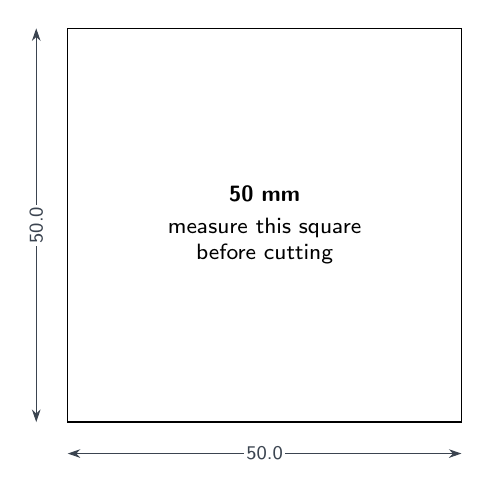
\begin{tikzpicture}[x=1mm,y=1mm]
    \draw[line width=0.5pt] (0,0) rectangle (50,50);
    \node[align=center,font=\footnotesize] at (25,25) {\textbf{50 mm}\\[2pt]measure this square\\before cutting};
    \draw[dim] (0,-4) -- (50,-4) node[dimlabel]{50.0};
    \draw[dim] (-4,0) -- (-4,50) node[dimlabel]{50.0};
  \end{tikzpicture}}

\newcommand{\code}[1]{\texttt{#1}}
\newcommand{\fig}[1]{Figure~\ref{#1}}

% ── running header and footer
\pagestyle{fancy}
\fancyhf{}
\renewcommand{\headrulewidth}{0.4pt}
\renewcommand{\headrule}{\hbox to\headwidth{\color{rule}\leaders\hrule height \headrulewidth\hfill}}
\fancyhead[L]{\footnotesize\color{muted}\doctitle}
\fancyhead[R]{\footnotesize\color{muted}radar-dev · 2.4 GHz FMCW radar}
\fancyfoot[L]{\footnotesize\color{muted}Sizes in mm unless marked. Generated from antenna/tools/horn.py and the 3-D model.}
\fancyfoot[R]{\footnotesize\color{muted}\thepage}
\fancypagestyle{plain}{\fancyhf{}\fancyfoot[R]{\footnotesize\color{muted}\thepage}\renewcommand{\headrulewidth}{0pt}}

% generated by tools/make_figures.py — do not edit
\newcommand{\aperW}{263.8}
\newcommand{\aperH}{193.1}
\newcommand{\pipeW}{86.4}
\newcommand{\pipeH}{43.2}
\newcommand{\flareL}{91.5}
\newcommand{\pipeL}{115}
\newcommand{\probeZ}{43.7}
\newcommand{\probeLen}{28}
\newcommand{\rodCut}{32}
\newcommand{\seam}{147.9}
\newcommand{\hTop}{118.3}
\newcommand{\hSide}{127.5}
\newcommand{\wideW}{87.5}
\newcommand{\backW}{88.5}
\newcommand{\backH}{44.3}
\newcommand{\tabW}{6}
\newcommand{\gain}{13.4}
\newcommand{\hpE}{34.2}
\newcommand{\hpH}{36.2}
\newcommand{\boardW}{457}
\newcommand{\boardD}{381}
\newcommand{\upH}{530.8}
\newcommand{\upX}{213}
\newcommand{\upCC}{426}
\newcommand{\beamLen}{444}
\newcommand{\beamRXlen}{408}
\newcommand{\beamRXtop}{252.8}
\newcommand{\beamTXtop}{542.8}
\newcommand{\rxY}{300}
\newcommand{\txY}{590}
\newcommand{\hornBase}{193.1}
\newcommand{\rowGap}{26.2}
\newcommand{\braceLen}{242.2}
\newcommand{\saddleW}{56.2}
\newcommand{\saddleGap}{48.2}
\newcommand{\saddleD}{34}
\newcommand{\saddleH}{32}
\newcommand{\saddleBehind}{90}
\newcommand{\overhang}{36}
\newcommand{\screenW}{293.1}
\newcommand{\screenH}{130}
\newcommand{\braceFootX}{128}
\newcommand{\txTop}{721.9}
\newcommand{\frontToFrame}{145.5}
\newcommand{\beamRXbottom}{240.8}
\newcommand{\braceTop}{226.8}
\newcommand{\leanTop}{39}
\newcommand{\leanSide}{44}
\newcommand{\cornerBend}{64}
\newcommand{\braceAngle}{69}
\newcommand{\sheetPct}{62}
\newcommand{\sheetIn}{178}

% table rows from a file: the primitive \input, because LaTeX's is not expandable inside a tabular
\makeatletter\newcommand{\rowsfrom}[1]{\@@input generated/#1.tex }\makeatother
\newcolumntype{Y}{>{\centering\arraybackslash}X}

\usepackage{needspace}
\graphicspath{{generated/}{../breadboard/assembly/steps/}}

% a breadboard step: the banner, kept with its picture
\newcommand{\bbstep}[2]{\par\needspace{85mm}\medskip
  \noindent\begin{tikzpicture}[baseline=(t.base)]
    \node[fill=logic,text=white,font=\bfseries,minimum width=9mm,minimum height=6mm,inner sep=2pt](n){B#1};
    \node[right=3mm of n.east,anchor=west,font=\large\bfseries](t){#2};
  \end{tikzpicture}\par\nopagebreak\smallskip}
% a phase gate
\newcommand{\gate}[1]{\begin{okbox}\textbf{\color{okgreen!70!black}Gate.}\ #1\end{okbox}}

\begin{document}

% ───────────────────────────────────────────────────────────── title page
\thispagestyle{plain}
\begin{tikzpicture}[remember picture,overlay]
  \fill[accent] (current page.north west) rectangle ([yshift=-9mm]current page.north east);
\end{tikzpicture}
\vspace*{6mm}
{\color{muted}\small radar-dev \quad·\quad 2.4 GHz FMCW radar \quad·\quad part 2 of 2}\par
\vspace{2mm}
{\fontsize{26}{30}\selectfont\bfseries Assembly and bring-up\par}
\vspace{1mm}
{\Large\color{accent} How it all goes together, and how to prove each stage works\par}
\vspace{5mm}
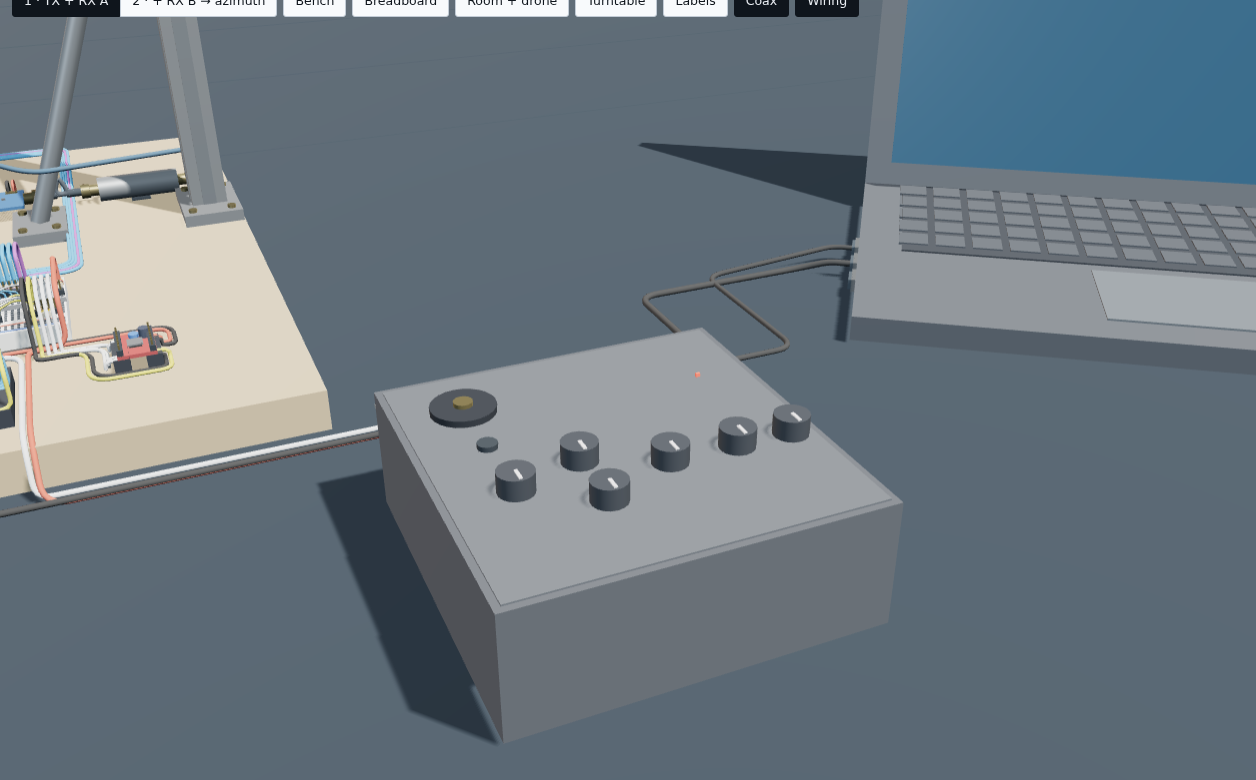
\includegraphics[width=\linewidth]{desk_view.png}\par
{\footnotesize\color{muted} The bench in use, from the 3-D model: horns on the frame, RF chain along the front of the board, the breadboard behind it, the sound card and laptop alongside.}
\vspace{4mm}

\begin{minipage}[t]{0.48\linewidth}
\textbf{Part 1} (fabrication) has the parts list, the copper templates, the frame drawings and the schematics. This part assumes you have the parts in hand and the pieces cut.

\smallskip
Work in the order of the stages. Each one ends with a \textbf{gate}: a measurement that must pass before you go on. A fault found at its own gate takes minutes; the same fault found at the end takes an evening.
\end{minipage}\hfill
\begin{minipage}[t]{0.48\linewidth}
\textbf{Conventions}
\begin{itemize}
  \item sizes in millimetres
  \item “left” and “right” are as you sit behind the bench, the horns pointing away from you into the room; “front” is the horn side
  \item \code{SWEEP 1} is something you type into the ESP32's serial monitor
  \item numbers like R4, C9, J12 match the schematics and the breadboard
\end{itemize}
\end{minipage}

\newpage
\tableofcontents
\newpage

% ───────────────────────────────────────────────────────────── 1 order
\section{The order of work}\label{sec:order}

Three jobs can run side by side while parts are arriving: the horns, the frame, and the breadboard. Everything after that is in series. The horns are the longest job; start them first.

\begin{figure}[H]
\centering
\begin{tikzpicture}[
  ph/.style={draw=black!60,fill=#1,rounded corners=1.5pt,minimum width=36mm,minimum height=11mm,align=center,font=\scriptsize},
  ph/.default=faint,
  g/.style={font=\tiny,text=okgreen!60!black,align=center},
  ar/.style={-{Stealth[length=2mm]},line width=0.7pt,draw=black!60}]
  \node[ph=cuout!50] (h) at (0,3.0) {\textbf{2. Three horns}\\a weekend};
  \node[ph=wood!70] (f) at (0,1.2) {\textbf{3. The frame}\\an afternoon};
  \node[ph=pcb] (b) at (0,-0.6) {\textbf{4. The breadboard}\\an evening};
  \node[ph] (p) at (5.2,-0.6) {\textbf{5. Power}\\buck to 5.00\,V};
  \node[ph] (fw) at (5.2,1.2) {\textbf{6. Firmware}\\\code{lock:1}};
  \node[ph=rfmod] (m) at (5.2,3.0) {\textbf{7. Mount and cable}\\horns, modules, SMA};
  \node[ph=okgreen!15] (l) at (10.4,3.0) {\textbf{8. First light}\\leakage tone, sync};
  \node[ph=okgreen!15] (w) at (10.4,1.2) {\textbf{9. First measurement}\\walk test, range};
  \node[ph=okgreen!15] (c) at (10.4,-0.6) {\textbf{10. Clutter, drone}\\the decision};
  \draw[ar] (b) -- (p);
  \draw[ar] (p) -- (fw);
  \draw[ar] (fw) -- (m);
  \draw[ar] (h.east) -- ++(0.5,0) |- ([yshift=2mm]m.west);
  \draw[ar] (f.east) -- ++(0.8,0) |- ([yshift=-2mm]m.west);
  \draw[ar] (m) -- (l);
  \draw[ar] (l) -- (w);
  \draw[ar] (w) -- (c);
  \node[g,below=0.5mm of h] {gate: record sheet, seams under 0.5\,Ω};
  \node[g,below=0.5mm of f] {gate: square, heights};
  \node[g,below=0.5mm of b] {gate: no shorts, power off};
  \node[g,below=0.5mm of p] {gate: 5.00\,V at J6, J7, J8};
  \node[g,below=0.5mm of fw] {gate: \code{lock:1}, \code{rf:0}};
  \node[g,below=0.5mm of m] {gate: every SMA torqued};
  \node[g,below=0.5mm of l] {gate: 26\,Hz tone, 135\,Hz square};
  \node[g,below=0.5mm of w] {gate: within 0.4\,m at 3, 5, 8\,m};
  \node[g,below=0.5mm of c] {gate: over 50\,dB, link LQ 100};
\end{tikzpicture}
\caption{The build in stages. Stages 2, 3 and 4 can be done in any order or at the same time; from stage 5 on, each needs the one before it.}
\end{figure}

{\small
\begin{tabularx}{\linewidth}{@{}p{6mm}P{0.22\linewidth}LP{0.25\linewidth}@{}}
\toprule
& \textbf{stage} & \textbf{what you end up with} & \textbf{the gate} \\ \midrule
2 & Three horns & three identical copper horns with connectors & each passes the record sheet \\
3 & The frame & plywood board, uprights, beams, saddles & square, beam tops at \beamRXtop\ and \beamTXtop \\
4 & The breadboard & the amplifier and power board, fully wired & no shorts between rails, power off \\
5 & Power & 5.00\,V to each module header, 12\,V to the op-amps & rail voltages in the table on page \pageref{sec:power} \\
6 & Firmware & the ESP32 talking to the PLL & \code{lock:1} with RF off \\
7 & Mount and cable & everything in place and connected & every SMA done up, still unpowered \\
8 & First light & the transmitter heard leaking into the receiver & a low tone with a ~26\,Hz part; a ~135\,Hz square wave \\
9 & First measurement & a person tracked across the room & range within 0.4\,m at 3, 5 and 8\,m \\
10 & Clutter and drone & the number that decides what the radar can see & clutter cancellation over 50\,dB \\
\bottomrule
\end{tabularx}}

\newpage
% ───────────────────────────────────────────────────────────── 2 horns
\section{Stage 2: the three horns}\label{sec:horns}

Make all three at once, step by step: cut all three sets, then fold all three, and so on. You get faster with every piece, and the two receive horns come out as twins, which matters later. Use the full-size templates in part 1.

\begin{figure}[H]
\centering
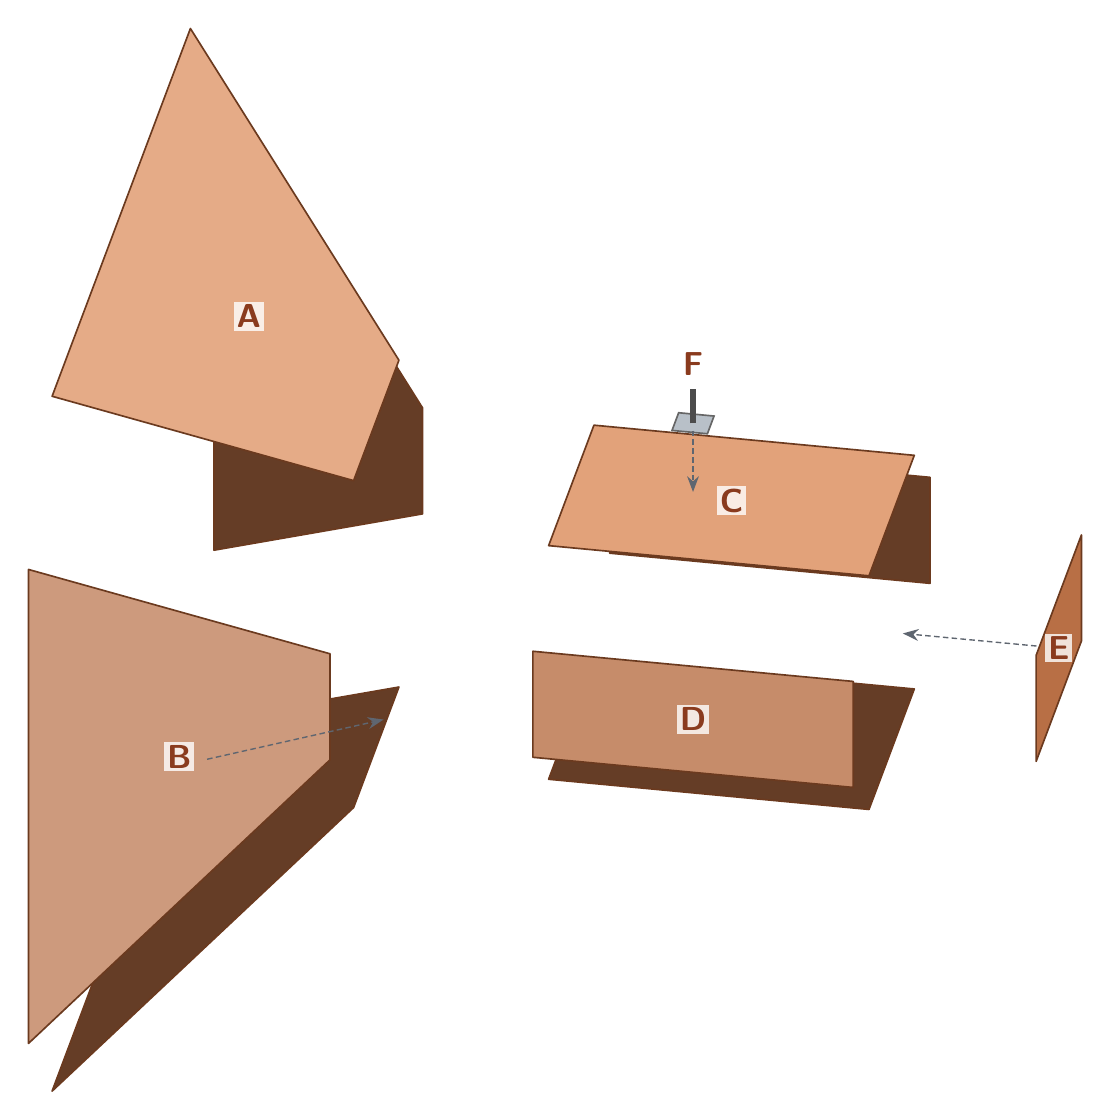
\begin{tikzpicture}[x=0.36mm,y=0.36mm]
\path[draw=cuedge,line width=0.6pt,line join=round,fill=cuin!55!black] (-165.49,41.81) -- (-165.49,79.21) -- (-239.05,196.21) -- (-239.05,29.00) -- cycle;
\path[draw=cuedge,line width=0.6pt,line join=round,fill=cuin!55!black] (-173.82,-19.28) -- (-189.80,-61.78) -- (-296.17,-161.83) -- (-247.38,-32.09) -- cycle;
\path[draw=cuedge,line width=0.6pt,line join=round,fill=cuin!55!black] (13.54,17.30) -- (13.54,54.70) -- (-99.47,65.35) -- (-99.47,27.95) -- cycle;
\path[draw=cuedge,line width=0.6pt,line join=round,fill=cuin!55!black] (7.99,-19.96) -- (-7.99,-62.46) -- (-121.01,-51.81) -- (-105.02,-9.32) -- cycle;
\path[draw=cuedge,line width=0.6pt,line join=round,fill=cuin] (66.96,-3.01) -- (50.97,-45.50) -- (50.97,-8.10) -- (66.96,34.39) -- cycle;
\node[font=\bfseries\large,text=accent,fill=white,fill opacity=0.8,text opacity=1,inner sep=1pt] at (58.96,-5.55) {E};
\path[draw=cuedge,line width=0.6pt,line join=round,fill=cuout] (7.99,62.46) -- (-7.99,19.96) -- (-121.01,30.61) -- (-105.02,73.10) -- cycle;
\node[font=\bfseries\large,text=accent,fill=white,fill opacity=0.8,text opacity=1,inner sep=1pt] at (-56.51,46.53) {C};
\path[draw=cuedge,line width=0.6pt,line join=round,fill=cuout!90] (-173.82,96.03) -- (-189.80,53.54) -- (-296.17,83.30) -- (-247.38,213.04) -- cycle;
\node[font=\bfseries\large,text=accent,fill=white,fill opacity=0.8,text opacity=1,inner sep=1pt] at (-226.79,111.48) {A};
\path[draw=cuedge,line width=0.6pt,line join=round,fill=cuin!80] (-13.54,-54.70) -- (-13.54,-17.30) -- (-126.56,-6.66) -- (-126.56,-44.06) -- cycle;
\node[font=\bfseries\large,text=accent,fill=white,fill opacity=0.8,text opacity=1,inner sep=1pt] at (-70.05,-30.68) {D};
\path[draw=cuedge,line width=0.6pt,line join=round,fill=cuin!70] (-198.12,-44.95) -- (-198.12,-7.55) -- (-304.50,22.20) -- (-304.50,-145.00) -- cycle;
\node[font=\bfseries\large,text=accent,fill=white,fill opacity=0.8,text opacity=1,inner sep=1pt] at (-251.31,-43.83) {B};
\draw[muted,line width=0.5pt,-{Stealth[length=2mm]},dash pattern=on 2pt off 1.2pt] (51.10,-4.81) -- (3.93,-0.37);
\draw[muted,line width=0.5pt,-{Stealth[length=2mm]},dash pattern=on 2pt off 1.2pt] (-241.48,-44.75) -- (-179.24,-30.75);
\path[alupart] (-62.65,76.32) -- (-65.00,70.07) -- (-77.48,71.25) -- (-75.14,77.49) -- cycle;
\path[draw=black!70,line width=2.4pt] (-70.07,73.78) -- (-70.07,85.90);
\draw[muted,line width=0.5pt,-{Stealth[length=2mm]},dash pattern=on 2pt off 1.2pt] (-70.07,71.19) -- (-70.07,49.54);
\node[font=\bfseries\large,text=accent] at (-70.07,94.56) {F};
\end{tikzpicture}

\caption{How the nine pieces and the connector go together. The pipe comes first (C, D, E), then the connector (F), then the flare (A, B) on the collar formed by the pipe's front tabs.}
\end{figure}

\step{Mark, cut and deburr}
\begin{note}[On a waterjet]
Cut the three sheets from \code{build/waterjet/horn\_sheet\_mm.dxf} as its README says, then skip to item 3 below: deburr and flatten. The feed hole in C is already cut, so step 2 is only the four flange holes.
\end{note}
\begin{enumerate}
  \item Tape the paper templates to the copper, outside face up, and scribe round them. Write each piece's letter on its outside face.
  \item Cut with the snips, blade just outside the line. Cut the angled ends of the B tabs and the notched corners of E last.
  \item File every edge smooth and flatten any piece the snips curled: lay it flat and press it with a block of wood.
\end{enumerate}
\checkline{every piece against its size in part 1, with calipers. A within 1\,mm on both parallel edges; both slanted edges of A and B \seam\ within 1\,mm.}

\step{Drill the feed hole while the top wall is flat}
\begin{enumerate}
  \item On \emph{one} C only, mark a point \probeZ\ up from the back edge and halfway across (\wideW/2 from either side). Centre-punch it.
  \item Drill a small pilot, then open it to 4.5\,mm so it clears the connector's white insulator. Deburr both sides.
  \item Hold the SMA flange over the hole, centred and square to the edges, and mark its four holes through it. Drill them 2.7\,mm.
\end{enumerate}
\checkline{the flange sits flat over the hole with its four screws through, and the centre pin is in the middle of the hole.}

\step{Fold the tabs}
Clamp the piece between two straight edges (angle iron or hardwood) with the fold line exactly on their edge, then press the tab over with a block of wood. Never fold by hand: it rounds the corner.

\begin{figure}[H]
\centering
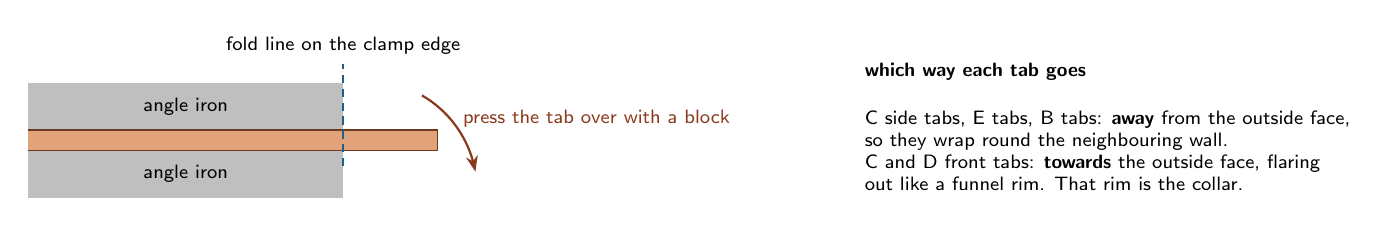
\begin{tikzpicture}[x=1mm,y=1mm,font=\scriptsize]
  % clamp
  \fill[black!25] (0,0) rectangle (40,6);
  \fill[black!25] (0,8.6) rectangle (40,14.6);
  \fill[cuout] (0,6) rectangle (52,8.6);
  \draw[cuedge] (0,6) -- (52,6) -- (52,8.6) -- (0,8.6);
  \draw[fold] (40,4) -- (40,17);
  \node[anchor=south] at (40,17) {fold line on the clamp edge};
  \node at (20,3) {angle iron};
  \node at (20,11.6) {angle iron};
  \draw[-{Stealth[length=2mm]},accent,line width=0.8pt] (50,13) arc[start angle=60,end angle=10,radius=14];
  \node[anchor=west,text=accent] at (54,10) {press the tab over with a block};
  % fold directions
  \begin{scope}[xshift=105mm]
    \node[anchor=west,font=\scriptsize\bfseries] at (0,16) {which way each tab goes};
    \node[anchor=west,align=left] at (0,6) {C side tabs, E tabs, B tabs: \textbf{away} from the outside face,\\so they wrap round the neighbouring wall.\\C and D front tabs: \textbf{towards} the outside face, flaring\\out like a funnel rim. That rim is the collar.};
  \end{scope}
\end{tikzpicture}
\end{figure}

\begin{tabularx}{\linewidth}{@{}P{0.2\linewidth}P{0.22\linewidth}L@{}}
\toprule
\textbf{piece} & \textbf{fold to} & \textbf{how to set it} \\ \midrule
C side tabs, E tabs & 90° & square against the clamp \\
B slanted-edge tabs & \cornerBend° & a card gauge cut to \cornerBend°; they lap over A at the corners \\
C front tabs & \leanTop° out & the card gauge on page \pageref{sec:gauges}; set later, at step 7 \\
D front tabs & \leanSide° out & the card gauge on page \pageref{sec:gauges}; set later, at step 7 \\
\bottomrule
\end{tabularx}

\step{Build the pipe}
\begin{figure}[H]
\centering
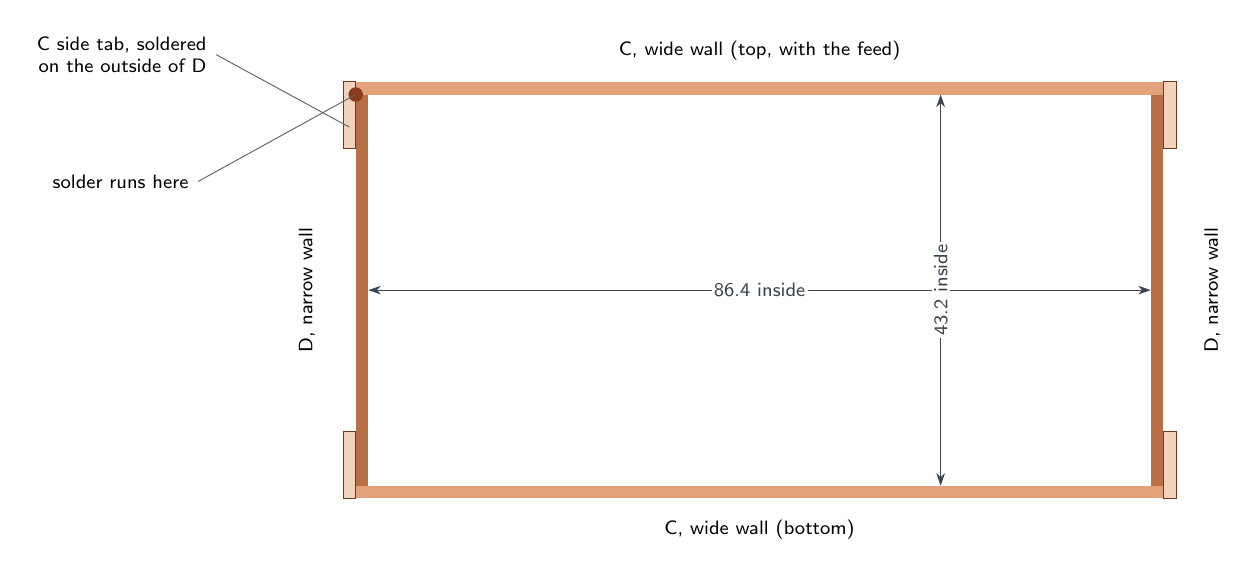
\begin{tikzpicture}[x=1.15mm,y=1.15mm,font=\scriptsize]
  \def\t{1.4}
  % D walls (narrow), standing
  \fill[cuin] (-43.2-\t,-21.6) rectangle (-43.2,21.6);
  \fill[cuin] (43.2,-21.6) rectangle (43.2+\t,21.6);
  % C walls (wide), with side tabs wrapping down over D
  \fill[cuout] (-43.2-\t,21.6) rectangle (43.2+\t,21.6+\t);
  \fill[cuout] (-43.2-\t,-21.6-\t) rectangle (43.2+\t,-21.6);
  \fill[tabfill,draw=cuedge,line width=0.3pt] (-43.2-2*\t,21.6+\t) rectangle (-43.2-\t,21.6-6);
  \fill[tabfill,draw=cuedge,line width=0.3pt] (43.2+\t,21.6+\t) rectangle (43.2+2*\t,21.6-6);
  \fill[tabfill,draw=cuedge,line width=0.3pt] (-43.2-2*\t,-21.6-\t) rectangle (-43.2-\t,-21.6+6);
  \fill[tabfill,draw=cuedge,line width=0.3pt] (43.2+\t,-21.6-\t) rectangle (43.2+2*\t,-21.6+6);
  \draw[dim] (-43.2,0) -- (43.2,0) node[dimlabel]{\pipeW\ inside};
  \draw[dim] (20,-21.6) -- (20,21.6) node[dimlabel]{\pipeH\ inside};
  \node at (0,26.5) {C, wide wall (top, with the feed)};
  \node at (0,-26.5) {C, wide wall (bottom)};
  \node[rotate=90] at (-50,0) {D, narrow wall};
  \node[rotate=90] at (50,0) {D, narrow wall};
  \draw[callout] (-43.2-1.5*\t,18) -- (-60,26) node[left,align=right]{C side tab, soldered\\on the outside of D};
  \fill[accent] (-43.2-\t,21.6) circle (0.8);
  \draw[callout] (-43.2-\t,21.6) -- (-62,12) node[left]{solder runs here};
\end{tikzpicture}
\caption{Looking into the pipe from the front, copper thickness exaggerated. The wide walls lap over the edges of the narrow ones; that is why C is cut \wideW, a little over \pipeW.}
\end{figure}
\begin{enumerate}
  \item Stand the two D walls on edge, \pipeW\ apart inside, and lay the bottom C across them with its side tabs folded down over their outsides. Clamp.
  \item Turn the box over and fit the top C, feed hole up, the same way.
  \item Measure inside at both ends with calipers: \pipeW\,×\,\pipeH, within half a millimetre, and the two diagonals equal. Adjust before any solder goes on.
  \item Tack each corner with a spot of solder, check again, then run solder along every tab from the outside. Keep the inside clean: solder blobs inside change the pipe's size.
\end{enumerate}

\step{Close the back}
Slide the back wall E over the back of the pipe, tabs forward over the outside, and solder all four tabs. The inside face of E is what the probe position is measured from, so it must sit flat and square across the whole end.
\checkline{inside, from the face of E to the centre of the feed hole: \probeZ\ ± 0.5.}

\step{Fit the connector and the probe}
\begin{enumerate}
  \item Cut \rodCut\ of brass rod and solder one end into the connector's centre cup, straight in line with it. If the rod will not enter the cup, file its end down until it does.
  \item Scrape the copper bright around the hole. Push the rod in through the hole and bolt the flange down tight with M2.5 screws: it must touch bare copper all round.
  \item Trim the rod so \probeLen\ stands inside, measured from the inside face of the wall. It must hang straight, square to the wall.
\end{enumerate}
\begin{note}[The probe is the one part worth tuning]
Its length and its distance from the back wall decide how much signal goes into the horn instead of bouncing back down the cable. If the HFSS model settles on different numbers, use those. To trim later, unbolt the connector and lift it out with the rod attached.
\end{note}

\step{Add the flare}
\begin{enumerate}
  \item Set the collar with the card gauges (page \pageref{sec:gauges}): the two C front tabs lean out \leanTop°, the two D front tabs \leanSide°.
  \item Set the top and bottom panels (A) on the C collar tabs, short edge to the pipe. Tack each at the middle of its short edge only.
  \item Set the side panels (B) on the D collar tabs, their slanted tabs over the outside of the A panels. Tack each at its short edge.
  \item Pull the corners together and tack each corner seam at the mouth.
  \item Measure the mouth at the rim: \aperW\,×\,\aperH\ inside, diagonals equal. Squeeze or spread the corners until it is, then tack the middle of each corner seam.
  \item Run the four corner seams and the collar, all from the outside, working from the pipe towards the mouth.
\end{enumerate}

\step{Check it, and fill in the record}
With a multimeter on its lowest resistance range, check every seam piece to piece, the connector body to the copper, and the centre pin to the copper. Then measure everything below.

{\small
\begin{tabularx}{\linewidth}{@{}P{0.34\linewidth}P{0.2\linewidth}YYY@{}}
\toprule
\textbf{check} & \textbf{target} & \textbf{horn 1 (TX)} & \textbf{horn 2 (RX)} & \textbf{horn 3 (spare RX)} \\ \midrule
mouth width, inside & \aperW\ ± 2 & & & \\
mouth height, inside & \aperH\ ± 2 & & & \\
mouth diagonals & equal ± 2 & & & \\
flare depth, mouth to pipe & \flareL\ ± 1 & & & \\
pipe inside & \pipeW\,×\,\pipeH\ ± 0.5 & & & \\
pipe length, back wall to flare & \pipeL\ ± 2 & & & \\
probe centre from back wall & \probeZ\ ± 0.5 & & & \\
probe length inside & \probeLen\ ± 0.5 & & & \\
every seam, piece to piece & under 0.5\,Ω & & & \\
connector body to copper & under 0.5\,Ω & & & \\
connector centre pin to copper & open & & & \\
\bottomrule
\end{tabularx}}

\gate{all three horns pass every line. The two that come out closest to each other are the receive horns; the third is the transmitter.}

\subsection*{Card gauges for the collar (full size)}\label{sec:gauges}
Trace onto card and cut out. Lay the long edge along the pipe wall; the slanted edge is where the front tab should be.
\begin{center}
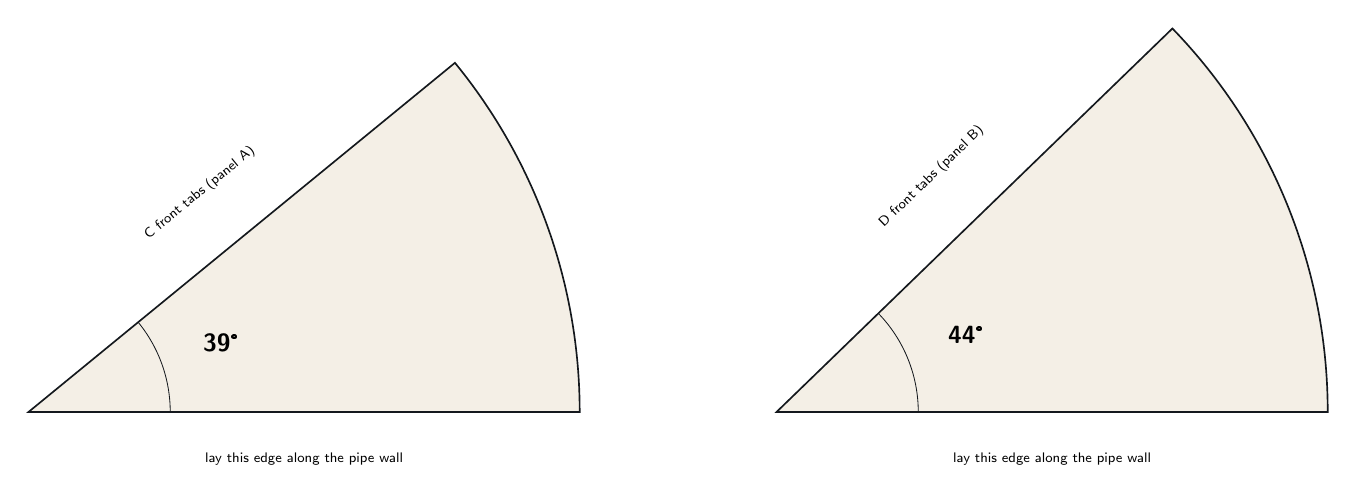
\begin{tikzpicture}[x=1.0mm,y=1.0mm]
\path[draw=ink,line width=0.6pt,fill=boxbg] (0.00,0.00) -- (70.00,0.00) arc[start angle=0,end angle=39.31,radius=70.0] -- cycle;
\draw[ink,line width=0.3pt] (18.00,0.00) arc[start angle=0,end angle=39.31,radius=18];
\node[font=\small] at (24.48,8.75) {\textbf{39°}};
\node[font=\tiny,anchor=north] at (35.00,-4.00) {lay this edge along the pipe wall};
\node[font=\tiny,rotate=39.31,anchor=south] at (23.08,26.17) {C front tabs (panel A)};
\path[draw=ink,line width=0.6pt,fill=boxbg] (95.00,0.00) -- (165.00,0.00) arc[start angle=0,end angle=44.09,radius=70.0] -- cycle;
\draw[ink,line width=0.3pt] (113.00,0.00) arc[start angle=0,end angle=44.09,radius=18];
\node[font=\small] at (119.10,9.76) {\textbf{44°}};
\node[font=\tiny,anchor=north] at (130.00,-4.00) {lay this edge along the pipe wall};
\node[font=\tiny,rotate=44.09,anchor=south] at (116.14,28.35) {D front tabs (panel B)};
\end{tikzpicture}

\end{center}

\newpage
% ───────────────────────────────────────────────────────────── 3 frame
\section{Stage 3: the frame}\label{sec:frame}

\begin{figure}[H]
\centering
\scalebox{0.8}{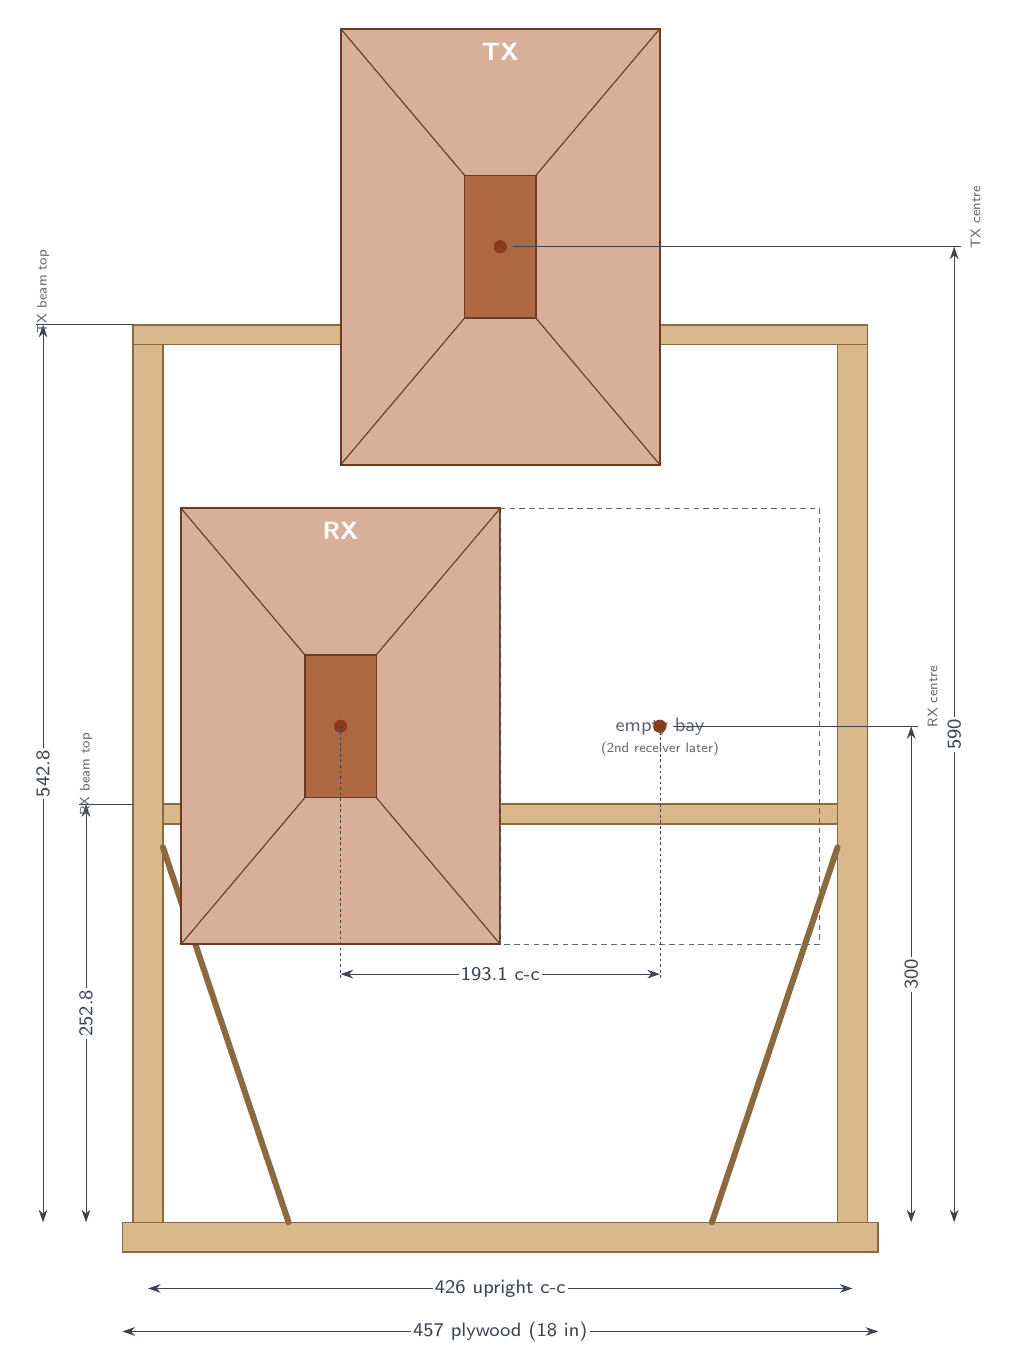
\begin{tikzpicture}[x=0.21mm,y=0.21mm]
\path[woodpart] (-228.50,-18.00) rectangle (228.50,0.00);
\path[woodpart] (-222.00,0.00) rectangle (-204.00,530.80);
\path[draw=woodedge,line width=2.2pt,line cap=round] (-204.00,226.80) -- (-128.00,0.00);
\path[woodpart] (204.00,0.00) rectangle (222.00,530.80);
\path[draw=woodedge,line width=2.2pt,line cap=round] (204.00,226.80) -- (128.00,0.00);
\path[woodpart] (-204.00,240.80) rectangle (204.00,252.80);
\path[woodpart] (-222.00,530.80) rectangle (222.00,542.80);
\path[draw=cuedge,line width=0.7pt,fill=cuin!55] (-193.12,168.11) rectangle (0.02,431.89);
\path[draw=cuedge,line width=0.5pt,fill=cuin!95!black] (-118.15,256.80) rectangle (-74.95,343.20);
\path[draw=cuedge,line width=0.4pt] (-74.95,343.20) -- (0.02,431.89);
\path[draw=cuedge,line width=0.4pt] (-74.95,256.80) -- (0.02,168.11);
\path[draw=cuedge,line width=0.4pt] (-118.15,343.20) -- (-193.12,431.89);
\path[draw=cuedge,line width=0.4pt] (-118.15,256.80) -- (-193.12,168.11);
\node[font=\bfseries\small,text=white] at (-96.55,417.89) {RX};
\fill[accent] (-96.55,300.00) circle[radius=4];
\path[hidden] (-0.02,168.11) rectangle (193.12,431.89);
\node[font=\scriptsize,text=muted,align=center] at (96.55,300.00) {empty bay};
\node[font=\tiny,text=muted] at (96.55,286.00) {(2nd receiver later)};
\fill[accent] (96.55,300.00) circle[radius=4];
\path[draw=cuedge,line width=0.7pt,fill=cuin!55] (-96.57,458.11) rectangle (96.57,721.89);
\path[draw=cuedge,line width=0.5pt,fill=cuin!95!black] (-21.60,546.80) rectangle (21.60,633.20);
\path[draw=cuedge,line width=0.4pt] (21.60,633.20) -- (96.57,721.89);
\path[draw=cuedge,line width=0.4pt] (21.60,546.80) -- (96.57,458.11);
\path[draw=cuedge,line width=0.4pt] (-21.60,633.20) -- (-96.57,721.89);
\path[draw=cuedge,line width=0.4pt] (-21.60,546.80) -- (-96.57,458.11);
\node[font=\bfseries\small,text=white] at (0.00,707.89) {TX};
\fill[accent] (0.00,590.00) circle[radius=4];
\draw[dim] (-96.55,150.12) -- (96.55,150.12) node[dimlabel]{193.1 c-c};
\path[ext,dash pattern=on 1pt off 1pt] (-96.55,300.00) -- (-96.55,146.11);
\path[ext,dash pattern=on 1pt off 1pt] (96.55,300.00) -- (96.55,146.11);
\draw[dim] (248.51,0.00) -- (248.51,300.00) node[dimlabel]{300};
\draw[dim] (274.51,0.00) -- (274.51,590.00) node[dimlabel]{590};
\path[ext] (104.55,300.00) -- (252.50,300.00);
\path[ext] (8.00,590.00) -- (278.50,590.00);
\draw[dim] (-250.51,0.00) -- (-250.51,252.80) node[dimlabel]{252.8};
\draw[dim] (-276.51,0.00) -- (-276.51,542.80) node[dimlabel]{542.8};
\path[ext] (-222.00,252.80) -- (-254.50,252.80);
\path[ext] (-222.00,542.80) -- (-280.50,542.80);
\draw[dim] (-213.00,-39.99) -- (213.00,-39.99) node[dimlabel]{426 upright c-c};
\draw[dim] (-228.50,-65.99) -- (228.50,-65.99) node[dimlabel]{457 plywood (18 in)};
\node[font=\tiny,text=muted,rotate=90] at (261.50,318.00) {RX centre};
\node[font=\tiny,text=muted,rotate=90] at (287.50,608.00) {TX centre};
\node[font=\tiny,text=muted,rotate=90] at (-250.50,270.80) {RX beam top};
\node[font=\tiny,text=muted,rotate=90] at (-276.50,562.80) {TX beam top};
\end{tikzpicture}
}
\caption{The frame from behind, from where you sit, with the horns in place (drawing from part 1, reduced).}
\end{figure}

\step{Cut and mark}
\begin{enumerate}
  \item Cut the parts on the cut list in part 1: two uprights \upH, the TX beam \beamLen, the RX beam \beamRXlen, two braces about \braceLen\ (leave them long; cut to fit at step 4).
  \item On the plywood, draw the centre line front to back, and a line across \frontToFrame\ from the front edge. That is the frame line: the centre of both uprights sits on it, \upX\ either side of the centre line (\upCC\ apart).
  \item On each upright, mark the top of the RX beam at \beamRXtop\ from the foot.
\end{enumerate}

\step{Stand the uprights}
\begin{enumerate}
  \item Screw an L-bracket to the front face and another to the back face of each upright foot, flush with the end.
  \item Stand each upright on its mark and screw the brackets to the board. Check it is square to the board in both directions with a square, before the last screws go in.
\end{enumerate}

\step{Fit the beams}
\begin{enumerate}
  \item \textbf{RX beam:} cut a spacer stick exactly \beamRXbottom\ long. Stand it beside each upright to hold the beam at the right height while you fit it. The beam goes \emph{between} the uprights; drill a 3.5\,mm hole through each upright at the beam's centre, and drive a screw through it into a pilot hole in the beam's end.
  \item \textbf{TX beam:} sits on top of both uprights, its ends flush with their outside faces. Drill 3.5\,mm through the beam \upCC\ apart, centred, and screw down into pilot holes in the upright tops.
\end{enumerate}
\checkline{both beam tops are level, the RX beam top is \beamRXtop\ above the board and the TX beam top \beamTXtop. The two diagonals of the frame (foot of one upright to the top of the other) are equal within 2\,mm.}

\step{Braces, saddles and the screen}
\begin{enumerate}
  \item Hold each brace against the inside of its upright, top end \braceTop\ above the board, foot on the board \braceFootX\ from the centre line. Mark both ends, cut them, and screw them in.
  \item Screw the saddles to the beams: on the RX beam two of them, centred 96.55 either side of the centre line (\hornBase\ apart); on the TX beam one, on the centre line. The U openings face up and run front to back.
  \item Make the foil screen: card \screenW\,×\,\screenH, foil on one side. Stand it 50\,mm behind the frame, centred, foil towards the horns.
\end{enumerate}
\gate{the frame does not rock on the bench, the saddle centres are where the drawing says, and a horn pipe drops into each saddle without forcing.}

\newpage
% ───────────────────────────────────────────────────────────── 4 breadboard
\section{Stage 4: the breadboard}\label{sec:bb}

Seventeen steps. Each adds a handful of parts, ends with something you can measure, and has a picture of the board as it should look afterwards. Power first so later stages have something to run on, then the op-amps, then the signal left to right, then the logic. Nothing is soldered; everything pushes in.

\begin{note}[Reading the hole names]
Columns 1–63 run left to right; rows a–e are the top bank, f–j the bottom. The five holes of one column in one bank are joined. \code{b14} is row b, column 14. \code{TR-@12} is the \textbf{top blue} rail nearest column 12. The rails: top red 5\,V, top blue GND, bottom red VANA (12\,V analogue), bottom blue GND. Wire colours follow the colour code in part 1.
\end{note}

\bbstep{1}{Rails, bridged and tied}
\begin{center}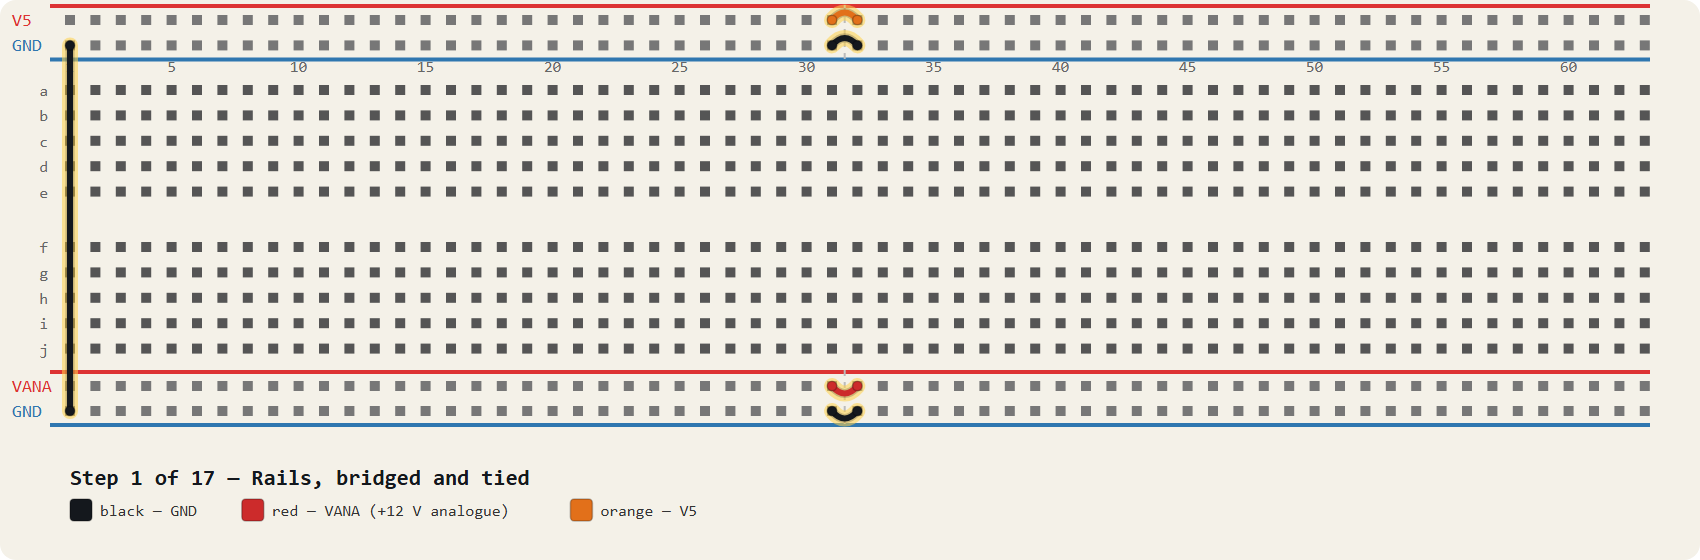
\includegraphics[width=\linewidth]{step-01.png}\end{center}
\vspace{-4pt}Nothing works until the four rails carry what they claim. Many 830-point boards split every rail at the middle, so the right-hand half of each is dead until you bridge it — and a split you did not notice is the classic reason half a board is unpowered. The last wire ties the two GND rails into one ground.\par
{\footnotesize \begin{tabular}{P{0.06\linewidth}P{0.12\linewidth}P{0.3\linewidth}P{0.42\linewidth}}
\toprule
\textbf{wire} & \textbf{colour} & \textbf{from → to} & \textbf{what it does}\\
\midrule
1 & orange & \textbf{TR+@31} → \textbf{TR+@32} & rail bridge (omit if your rails are continuous)\\
2 & black & \textbf{TR-@31} → \textbf{TR-@32} & rail bridge\\
3 & red & \textbf{BR+@31} → \textbf{BR+@32} & rail bridge\\
4 & black & \textbf{BR-@31} → \textbf{BR-@32} & rail bridge\\
5 & black & \textbf{TR-@1} → \textbf{BR-@1} & tie the two GND rails together\\
\bottomrule
\end{tabular}}\par
\checkline{Continuity from each rail's far left hole to its far right hole. If your board's rails are continuous, these four bridges are harmless.}
\bbstep{2}{12 V in, and the diode that saves the board}
\begin{center}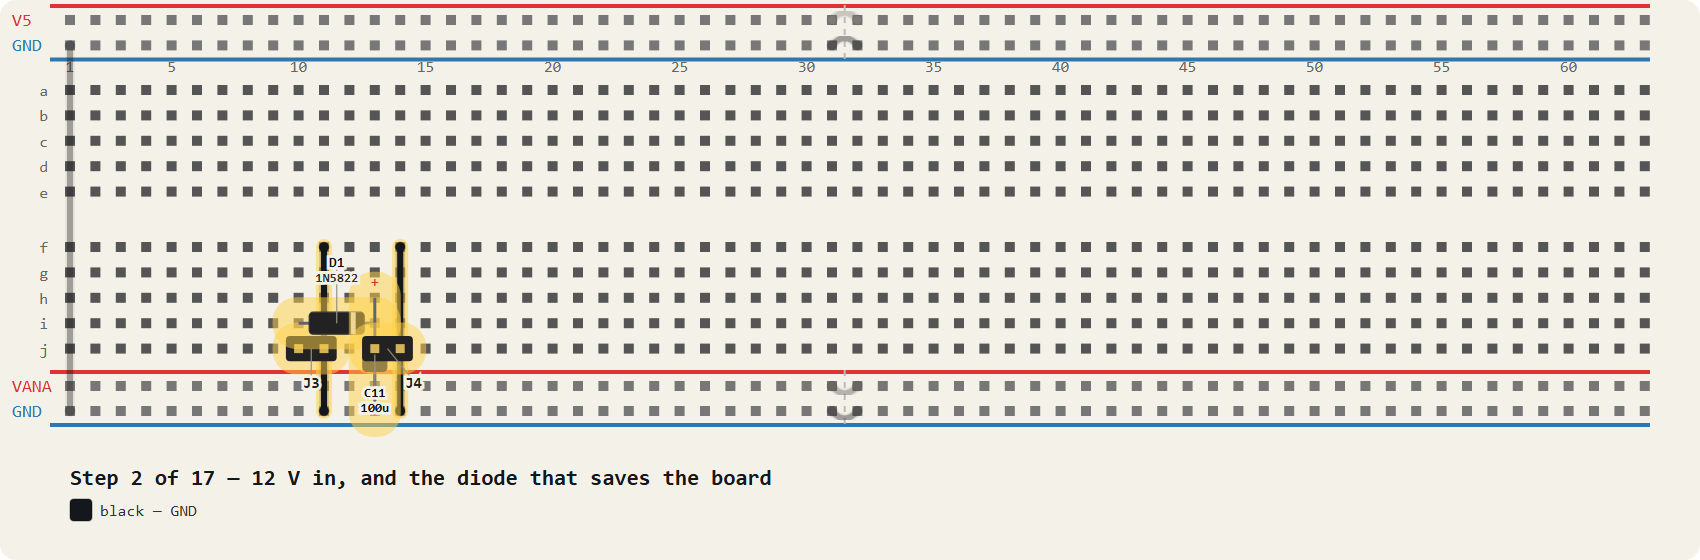
\includegraphics[width=\linewidth]{step-02.png}\end{center}
\vspace{-4pt}J3 takes the 12 V supply. D1 is a series Schottky: get the supply backwards and it simply does not conduct, instead of taking the op-amps and the electrolytics with it. The band on the diode body is the cathode and it faces RIGHT, toward column 13. C11 is the bulk reservoir on the protected side.\par
{\footnotesize \begin{tabular}{P{0.12\linewidth}P{0.22\linewidth}P{0.56\linewidth}}
\toprule
\textbf{part} & \textbf{value} & \textbf{push it in at}\\
\midrule
J3 & 12V IN & 1→\textbf{j10}, 2→\textbf{j11}\\
D1 & 1N5822 & A→\textbf{i10}, K→\textbf{i13}\\
C11 & 100u & 1→\textbf{h13}, 2→\textbf{BR-@13}\\
J4 & TO BUCK IN & 1→\textbf{j13}, 2→\textbf{j14}\\
\bottomrule
\end{tabular}}\par
{\footnotesize \begin{tabular}{P{0.06\linewidth}P{0.12\linewidth}P{0.3\linewidth}P{0.42\linewidth}}
\toprule
\textbf{wire} & \textbf{colour} & \textbf{from → to} & \textbf{what it does}\\
\midrule
1 & black & \textbf{f11} → \textbf{BR-@11} & J3 GND\\
2 & black & \textbf{f14} → \textbf{BR-@14} & J4 GND\\
\bottomrule
\end{tabular}}\par
\checkline{D1's band toward column 13. C11's + leg toward column 13, its - to the GND rail.}
\bbstep{3}{The VANA rail — clean 12 V for the op-amps}
\begin{center}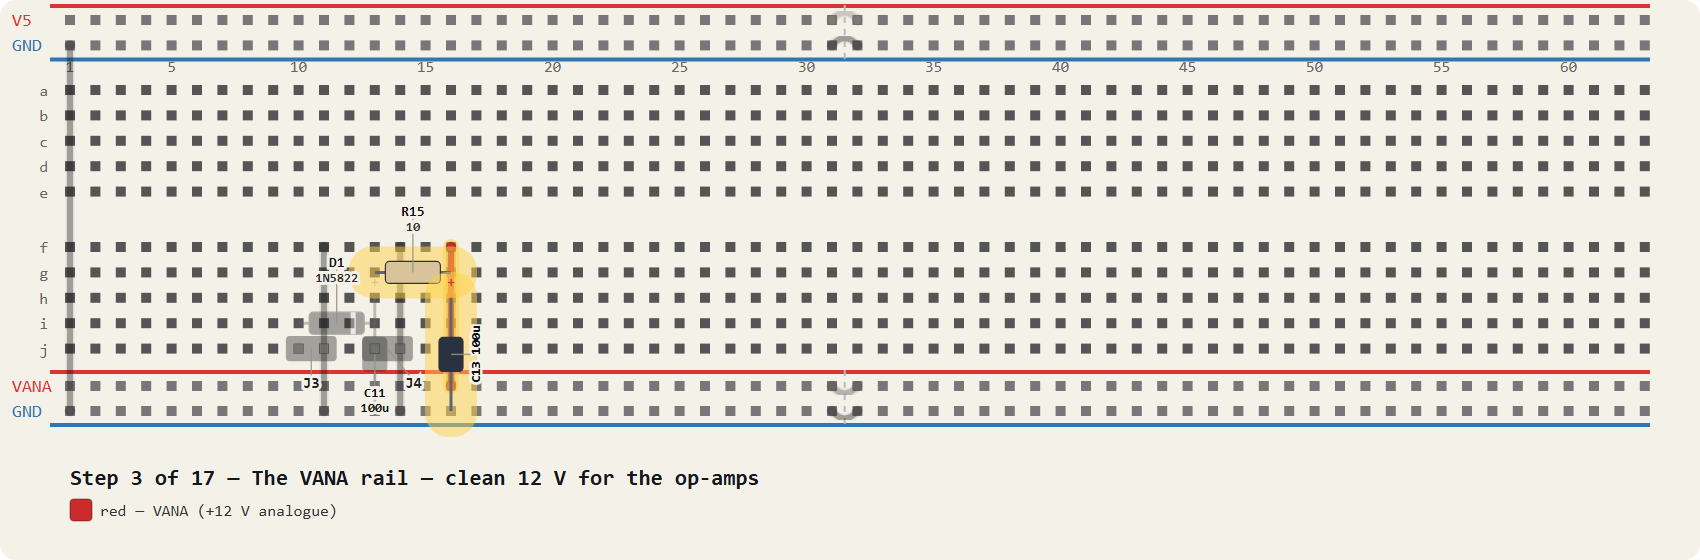
\includegraphics[width=\linewidth]{step-03.png}\end{center}
\vspace{-4pt}R15 and C13 are an RC filter, not a resistor someone forgot to remove: 10 ohms into 100 uF rolls off at about 160 Hz, which keeps supply noise out of an amplifier whose whole job is a signal down at 20 mV. The output of that filter is what feeds the bottom red rail.\par
{\footnotesize \begin{tabular}{P{0.12\linewidth}P{0.22\linewidth}P{0.56\linewidth}}
\toprule
\textbf{part} & \textbf{value} & \textbf{push it in at}\\
\midrule
R15 & 10 & 1→\textbf{g13}, 2→\textbf{g16}\\
C13 & 100u & 1→\textbf{h16}, 2→\textbf{BR-@16}\\
\bottomrule
\end{tabular}}\par
{\footnotesize \begin{tabular}{P{0.06\linewidth}P{0.12\linewidth}P{0.3\linewidth}P{0.42\linewidth}}
\toprule
\textbf{wire} & \textbf{colour} & \textbf{from → to} & \textbf{what it does}\\
\midrule
1 & red & \textbf{f16} → \textbf{BR+@16} & VANA node (R15/C13) feeds the bottom red rail\\
\bottomrule
\end{tabular}}\par
\checkline{Bottom red rail now sits at 12 V minus the diode drop, about 11.6 V.}
\bbstep{4}{5 V in from the buck converter}
\begin{center}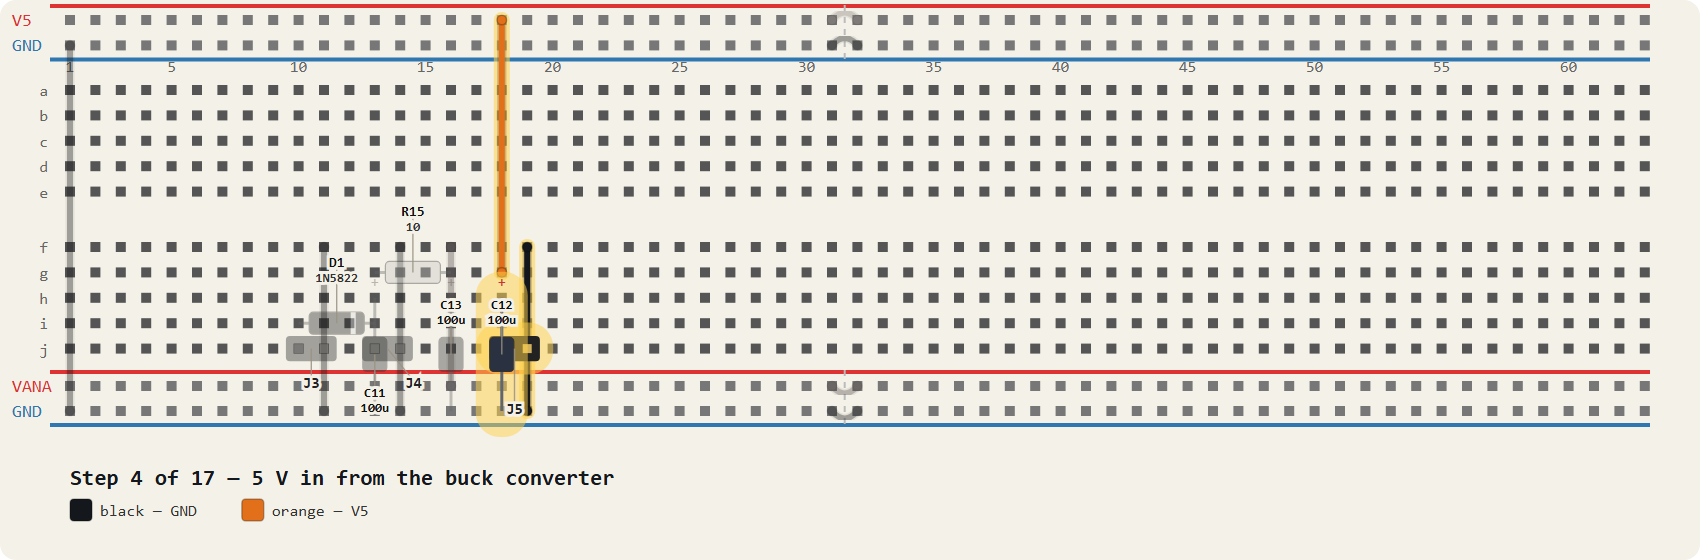
\includegraphics[width=\linewidth]{step-04.png}\end{center}
\vspace{-4pt}J5 brings 5 V back from the LM2596 after you have set it with nothing else connected. C12 decouples it and the orange wire carries it up to the top red rail, which is what the three RF modules will feed from.\par
{\footnotesize \begin{tabular}{P{0.12\linewidth}P{0.22\linewidth}P{0.56\linewidth}}
\toprule
\textbf{part} & \textbf{value} & \textbf{push it in at}\\
\midrule
J5 & FROM BUCK 5V & 1→\textbf{j18}, 2→\textbf{j19}\\
C12 & 100u & 1→\textbf{h18}, 2→\textbf{BR-@18}\\
\bottomrule
\end{tabular}}\par
{\footnotesize \begin{tabular}{P{0.06\linewidth}P{0.12\linewidth}P{0.3\linewidth}P{0.42\linewidth}}
\toprule
\textbf{wire} & \textbf{colour} & \textbf{from → to} & \textbf{what it does}\\
\midrule
1 & black & \textbf{f19} → \textbf{BR-@19} & J5 GND\\
2 & orange & \textbf{g18} → \textbf{TR+@18} & V5 (J5/C12, bottom col 18) up to the top red rail\\
\bottomrule
\end{tabular}}\par
\checkline{Set the buck to 5.00 V BEFORE this wire goes in. Top red rail = 5.00 V.}
\bbstep{5}{Seat the two op-amps}
\begin{center}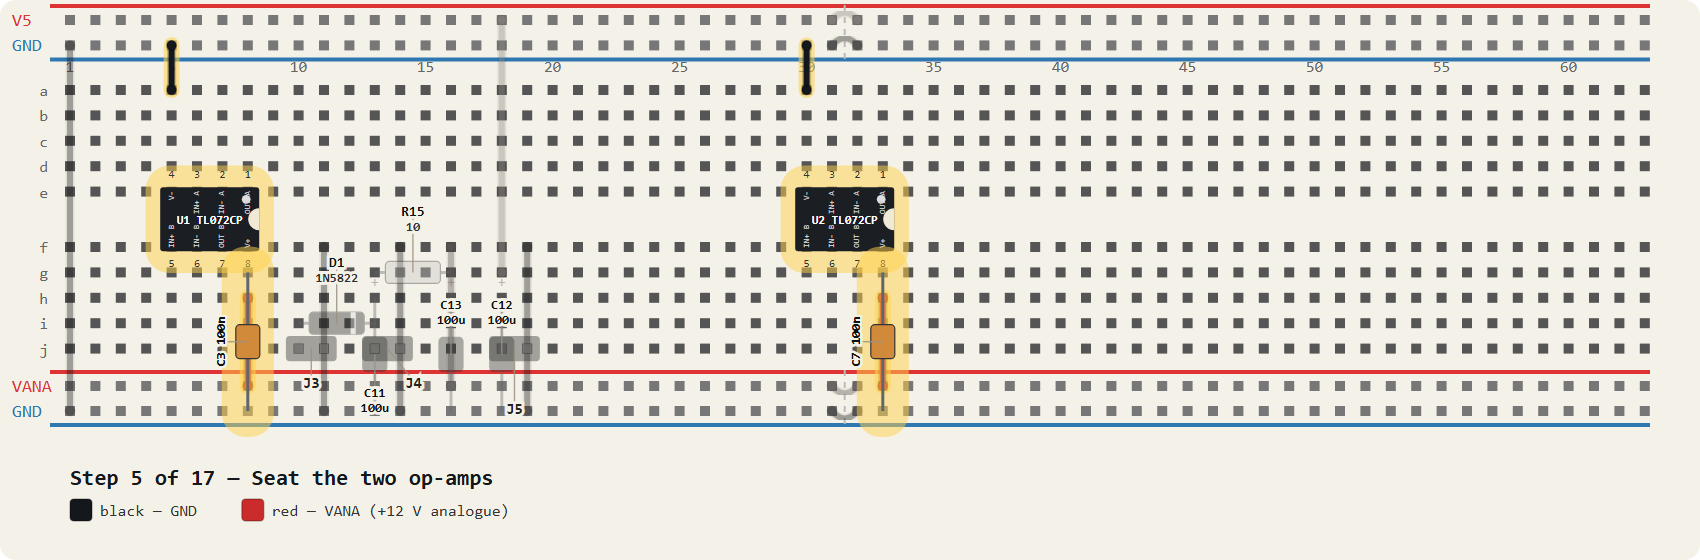
\includegraphics[width=\linewidth]{step-05.png}\end{center}
\vspace{-4pt}U1 is the two gain stages, U2 the reference buffer and the output. Both straddle the centre channel so the two sides of the package land on separate strips. The notch and the pin-1 dot face RIGHT, toward the higher column. C3 and C7 are the 100 nF decouplers and they go right at pin 8 of each chip, not somewhere tidier.\par
{\footnotesize \begin{tabular}{P{0.12\linewidth}P{0.22\linewidth}P{0.56\linewidth}}
\toprule
\textbf{part} & \textbf{value} & \textbf{push it in at}\\
\midrule
U1 & TL072CP & 4→\textbf{e5}, 3→\textbf{e6}, 2→\textbf{e7}, 1→\textbf{e8}, 5→\textbf{f5}, 6→\textbf{f6}, 7→\textbf{f7}, 8→\textbf{f8}\\
U2 & TL072CP & 4→\textbf{e30}, 3→\textbf{e31}, 2→\textbf{e32}, 1→\textbf{e33}, 5→\textbf{f30}, 6→\textbf{f31}, 7→\textbf{f32}, 8→\textbf{f33}\\
C3 & 100n & 1→\textbf{g8}, 2→\textbf{BR-@8}\\
C7 & 100n & 1→\textbf{g33}, 2→\textbf{BR-@33}\\
\bottomrule
\end{tabular}}\par
{\footnotesize \begin{tabular}{P{0.06\linewidth}P{0.12\linewidth}P{0.3\linewidth}P{0.42\linewidth}}
\toprule
\textbf{wire} & \textbf{colour} & \textbf{from → to} & \textbf{what it does}\\
\midrule
1 & black & \textbf{a5} → \textbf{TR-@5} & U1 pin 4 (V-, top col 5) to the GND rail\\
2 & black & \textbf{a30} → \textbf{TR-@30} & U2 pin 4 (V-, top col 30) to the GND rail\\
3 & red & \textbf{h8} → \textbf{BR+@8} & U1 pin 8 (V+, bottom col 8) to the VANA rail\\
4 & red & \textbf{h33} → \textbf{BR+@33} & U2 pin 8 (V+, bottom col 33) to the VANA rail\\
\bottomrule
\end{tabular}}\par
\checkline{Pin 1 at e8 (U1) and e33 (U2). Power the board: both chips should sit at room temperature. A warm op-amp means V+ and V- are swapped.}
\bbstep{6}{The half-rail reference}
\begin{center}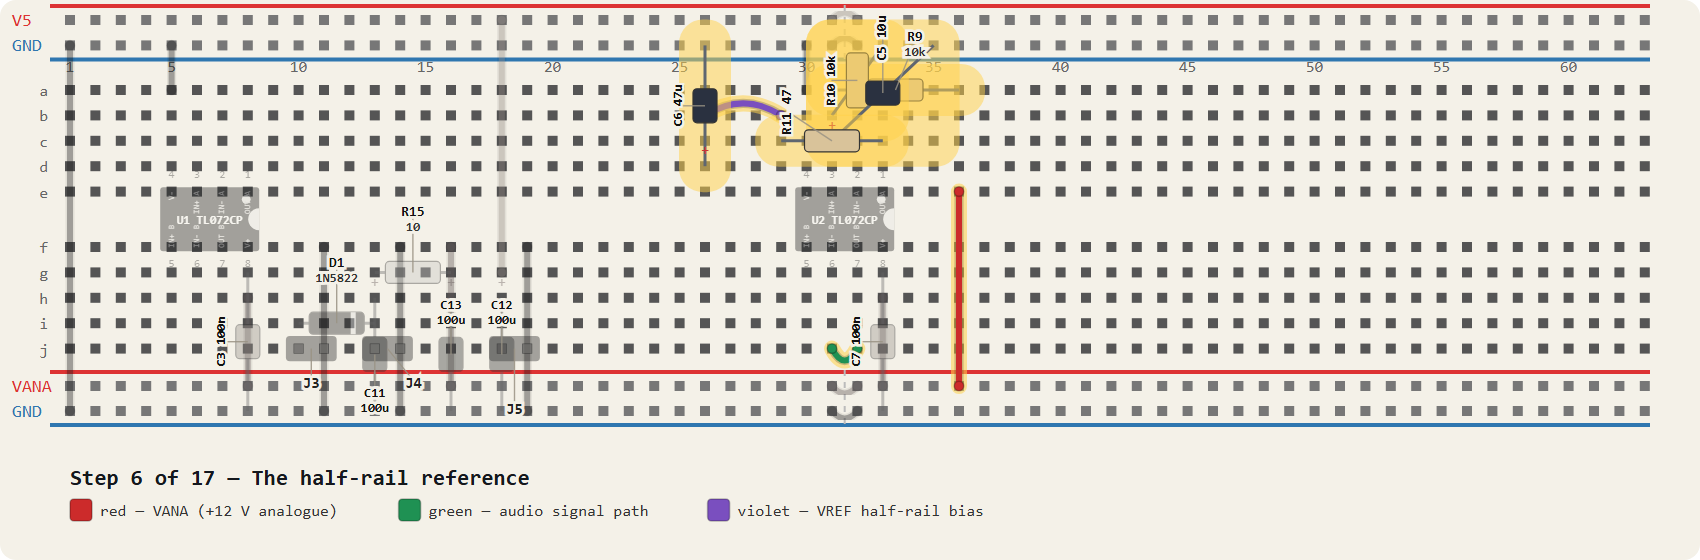
\includegraphics[width=\linewidth]{step-06.png}\end{center}
\vspace{-4pt}This amplifier runs on a single supply, so 'zero' has to be manufactured: R9 and R10 divide VANA in half at column 31, C5 holds it still, and U2's second half buffers it so the divider is not loaded by everything downstream. R11 and C6 carry that buffered VREF to the node the whole signal chain hangs off.\par
{\footnotesize \begin{tabular}{P{0.12\linewidth}P{0.22\linewidth}P{0.56\linewidth}}
\toprule
\textbf{part} & \textbf{value} & \textbf{push it in at}\\
\midrule
R9 & 10k & 1→\textbf{a36}, 2→\textbf{a31}\\
R10 & 10k & 1→\textbf{b31}, 2→\textbf{TR-@33}\\
C5 & 10u & 1→\textbf{c31}, 2→\textbf{TR-@35}\\
R11 & 47 & 1→\textbf{c33}, 2→\textbf{c29}\\
C6 & 47u & 1→\textbf{d26}, 2→\textbf{TR-@26}\\
\bottomrule
\end{tabular}}\par
{\footnotesize \begin{tabular}{P{0.06\linewidth}P{0.12\linewidth}P{0.3\linewidth}P{0.42\linewidth}}
\toprule
\textbf{wire} & \textbf{colour} & \textbf{from → to} & \textbf{what it does}\\
\midrule
1 & red & \textbf{e36} → \textbf{BR+@36} & R9's VANA end (top col 36) down to the VANA rail\\
2 & green & \textbf{j32} → \textbf{j31} & U2 pin 7 (col 32) to pin 6 (col 31): unity-gain buffer\\
3 & green & \textbf{a33} → \textbf{a32} & U2 pin 1 (col 33) to pin 2 (col 32): VREF buffer, unity gain\\
4 & violet & \textbf{b29} → \textbf{b26} & R11's far end (col 29) to the VREF node (col 26)\\
\bottomrule
\end{tabular}}\par
\checkline{VREF (column 26) should read half of VANA, about 5.8 V, and be steady.}
\bbstep{7}{Spread VREF along the board}
\begin{center}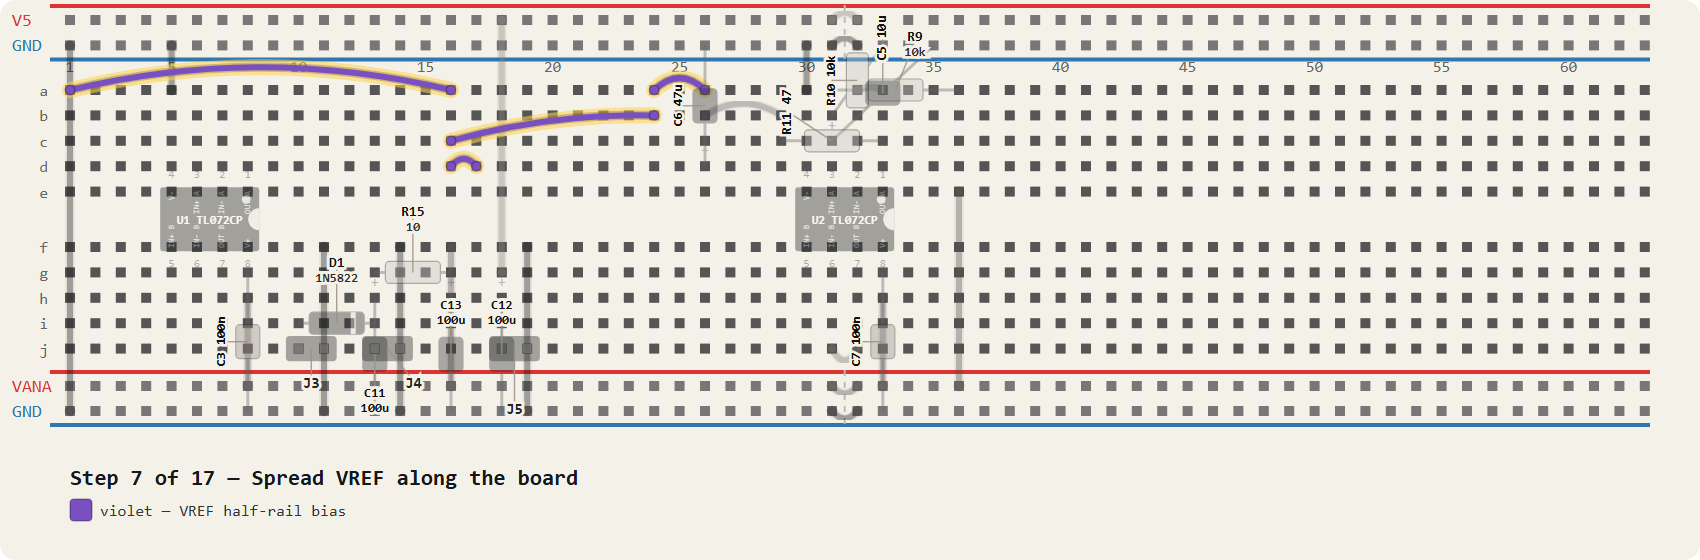
\includegraphics[width=\linewidth]{step-07.png}\end{center}
\vspace{-4pt}Four violet wires, and they are the reason the amplifier has a zero to swing about. The long one runs the length of row a to reach the input stage at column 1. Do them as a set so none is forgotten — a stage whose VREF is missing is not dead, it is railed, which is a more confusing symptom.\par
{\footnotesize \begin{tabular}{P{0.06\linewidth}P{0.12\linewidth}P{0.3\linewidth}P{0.42\linewidth}}
\toprule
\textbf{wire} & \textbf{colour} & \textbf{from → to} & \textbf{what it does}\\
\midrule
1 & violet & \textbf{a26} → \textbf{a24} & VREF -> C9's VREF end\\
2 & violet & \textbf{b24} → \textbf{c16} & VREF -> R6's VREF end (col 16)\\
3 & violet & \textbf{d16} → \textbf{d17} & VREF (col 16) -> R4's VREF end (col 17)\\
4 & violet & \textbf{a1} → \textbf{a16} & VREF -> R2's VREF end (col 1): long run along row a\\
\bottomrule
\end{tabular}}\par
\checkline{Every violet wire end reads the same 5.8 V.}
\bbstep{8}{The input: mixer IF, terminated}
\begin{center}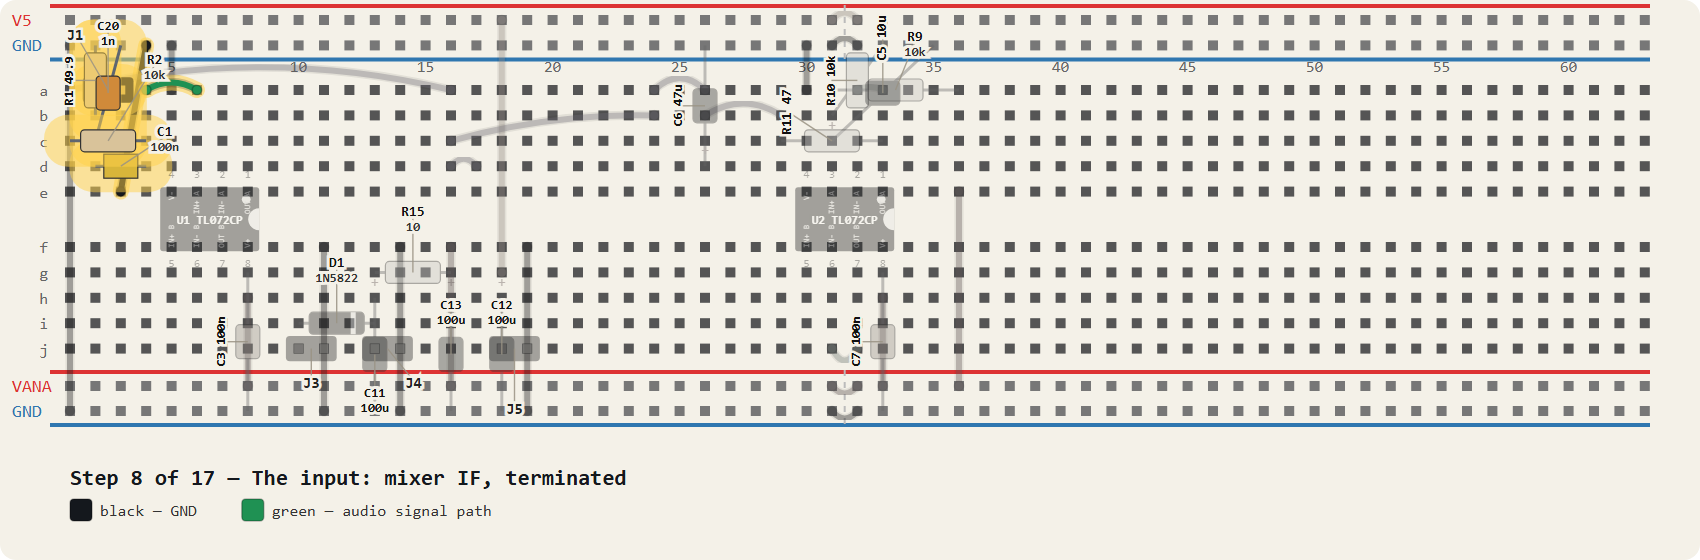
\includegraphics[width=\linewidth]{step-08.png}\end{center}
\vspace{-4pt}R1 is the 49.9 ohm load the mixer's IF port wants; without it the conversion loss and the flatness wander. C20 shunts the LO that leaks out of that same port at 2.4 GHz, which a TL072 would otherwise rectify into a DC offset. C1 and R2 are the first high-pass, and they are what stop the TX leakage tone from saturating the gain.\par
{\footnotesize \begin{tabular}{P{0.12\linewidth}P{0.22\linewidth}P{0.56\linewidth}}
\toprule
\textbf{part} & \textbf{value} & \textbf{push it in at}\\
\midrule
J1 & MIXER IF & 1→\textbf{a2}, 2→\textbf{a3}\\
R1 & 49.9 & 1→\textbf{b2}, 2→\textbf{TR-@2}\\
C20 & 1n & 1→\textbf{c2}, 2→\textbf{TR-@3}\\
C1 & 100n & 1→\textbf{d2}, 2→\textbf{d4}\\
R2 & 10k & 1→\textbf{c4}, 2→\textbf{c1}\\
\bottomrule
\end{tabular}}\par
{\footnotesize \begin{tabular}{P{0.06\linewidth}P{0.12\linewidth}P{0.3\linewidth}P{0.42\linewidth}}
\toprule
\textbf{wire} & \textbf{colour} & \textbf{from → to} & \textbf{what it does}\\
\midrule
1 & black & \textbf{e3} → \textbf{TR-@4} & J1 GND\\
2 & green & \textbf{a4} → \textbf{a6} & AP (C1/R2 node) into U1 pin 3 (IN+ A, col 6)\\
\bottomrule
\end{tabular}}\par
\checkline{R1 across the IF input reads 49.9 ohms to ground.}
\bbstep{9}{Gain stage A, times 101}
\begin{center}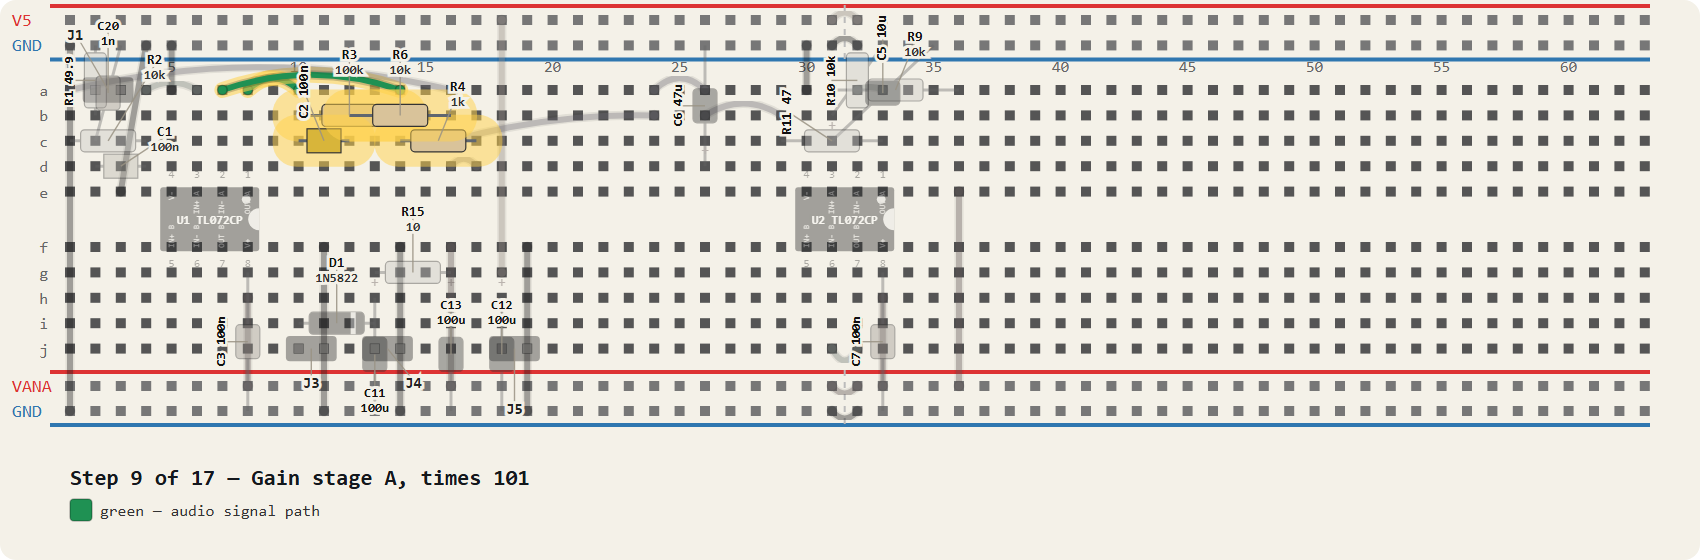
\includegraphics[width=\linewidth]{step-09.png}\end{center}
\vspace{-4pt}R3 over R4 sets the gain. R4 is 1k for the full 40 dB, but fit 4.7k on first power-up for a gain of 22: if the TX leakage is stronger than you expected, a lower first gain is the difference between seeing it and clipping on it. C2 and R6 are the second high-pass into stage B.\par
{\footnotesize \begin{tabular}{P{0.12\linewidth}P{0.22\linewidth}P{0.56\linewidth}}
\toprule
\textbf{part} & \textbf{value} & \textbf{push it in at}\\
\midrule
R3 & 100k & 1→\textbf{b14}, 2→\textbf{b10}\\
C2 & 100n & 1→\textbf{c10}, 2→\textbf{c12}\\
R4 & 1k & 1→\textbf{c14}, 2→\textbf{c17}\\
R6 & 10k & 1→\textbf{b12}, 2→\textbf{b16}\\
\bottomrule
\end{tabular}}\par
{\footnotesize \begin{tabular}{P{0.06\linewidth}P{0.12\linewidth}P{0.3\linewidth}P{0.42\linewidth}}
\toprule
\textbf{wire} & \textbf{colour} & \textbf{from → to} & \textbf{what it does}\\
\midrule
1 & green & \textbf{a8} → \textbf{a10} & U1 pin 1 (OUT A, col 8) to the AOUT node (col 10)\\
2 & green & \textbf{a14} → \textbf{a7} & AM node (R3/R4) back to U1 pin 2 (IN- A, col 7)\\
\bottomrule
\end{tabular}}\par
\checkline{Inject 10 mV at 1 kHz: about 107 mV out of stage A with R4 at 4.7k.}
\bbstep{10}{Gain stage B, times 11, and the anti-alias corner}
\begin{center}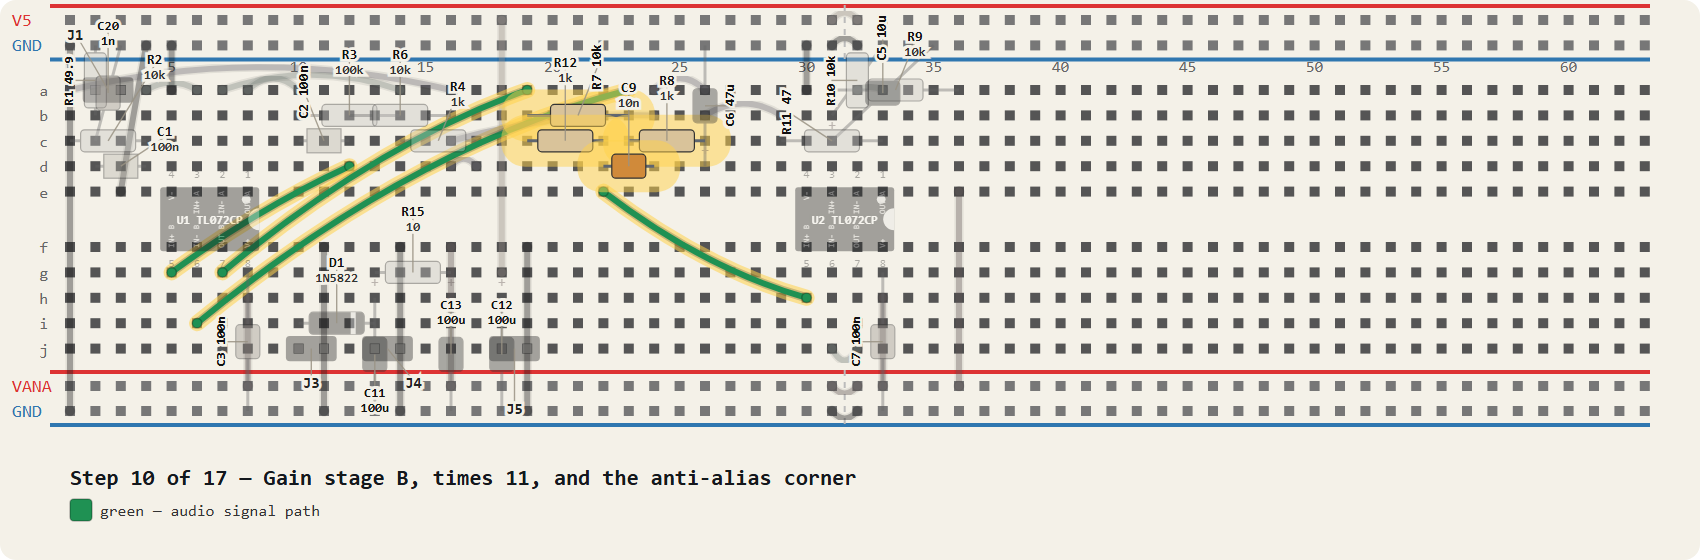
\includegraphics[width=\linewidth]{step-10.png}\end{center}
\vspace{-4pt}R7 over R8 gives the second 21 dB. R12 with C9 is the 15.9 kHz low-pass that limits the noise bandwidth reaching the sound card. The last wire takes that filtered node across the channel into U2's spare half.\par
{\footnotesize \begin{tabular}{P{0.12\linewidth}P{0.22\linewidth}P{0.56\linewidth}}
\toprule
\textbf{part} & \textbf{value} & \textbf{push it in at}\\
\midrule
R7 & 10k & 1→\textbf{b23}, 2→\textbf{b19}\\
R8 & 1k & 1→\textbf{c23}, 2→\textbf{c26}\\
R12 & 1k & 1→\textbf{c19}, 2→\textbf{c22}\\
C9 & 10n & 1→\textbf{d22}, 2→\textbf{d24}\\
\bottomrule
\end{tabular}}\par
{\footnotesize \begin{tabular}{P{0.06\linewidth}P{0.12\linewidth}P{0.3\linewidth}P{0.42\linewidth}}
\toprule
\textbf{wire} & \textbf{colour} & \textbf{from → to} & \textbf{what it does}\\
\midrule
1 & green & \textbf{d12} → \textbf{g5} & BP (C2/R6 node) across the channel into U1 pin 5 (IN+ B, bottom col 5)\\
2 & green & \textbf{g7} → \textbf{a19} & U1 pin 7 (OUT B, bottom col 7) up to the BOUT node (col 19)\\
3 & green & \textbf{a23} → \textbf{i6} & BM node (R7/R8) across to U1 pin 6 (IN- B, bottom col 6)\\
4 & green & \textbf{e22} → \textbf{h30} & LP (R12/C9 node) across to U2 pin 5 (IN+ B, bottom col 30)\\
\bottomrule
\end{tabular}}\par
\checkline{Total gain now about 61 dB. Sweep it: -3 dB at 15.9 kHz, -6 dB at 159 Hz.}
\bbstep{11}{Output, isolated and bled to ground}
\begin{center}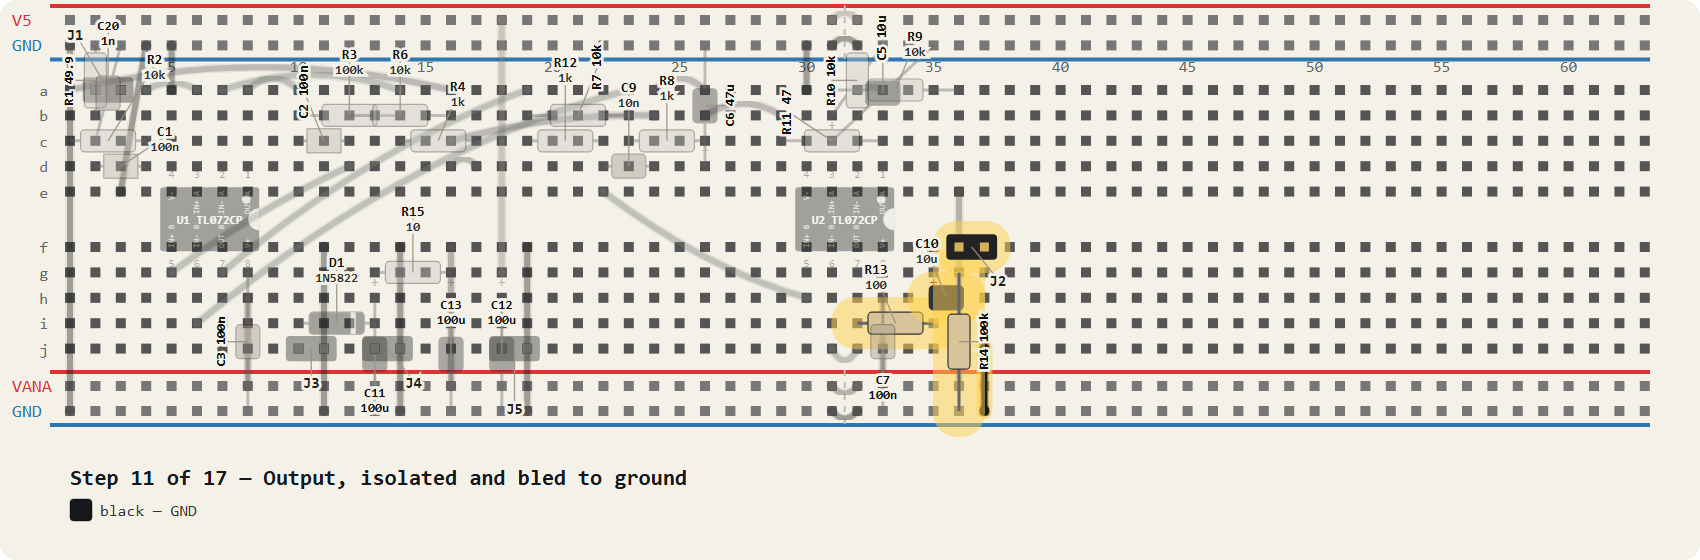
\includegraphics[width=\linewidth]{step-11.png}\end{center}
\vspace{-4pt}R13 and C10 hand the signal to the sound card through a series resistor, so a cable capacitance does not hang directly off an op-amp output. R14 bleeds the coupling cap so the jack is not left holding a charge, and J2 is the audio-left output to the interface.\par
{\footnotesize \begin{tabular}{P{0.12\linewidth}P{0.22\linewidth}P{0.56\linewidth}}
\toprule
\textbf{part} & \textbf{value} & \textbf{push it in at}\\
\midrule
R13 & 100 & 1→\textbf{i32}, 2→\textbf{i35}\\
C10 & 10u & 1→\textbf{h35}, 2→\textbf{h36}\\
R14 & 100k & 1→\textbf{g36}, 2→\textbf{BR-@36}\\
J2 & AUDIO L & 1→\textbf{f36}, 2→\textbf{f37}\\
\bottomrule
\end{tabular}}\par
{\footnotesize \begin{tabular}{P{0.06\linewidth}P{0.12\linewidth}P{0.3\linewidth}P{0.42\linewidth}}
\toprule
\textbf{wire} & \textbf{colour} & \textbf{from → to} & \textbf{what it does}\\
\midrule
1 & black & \textbf{j37} → \textbf{BR-@37} & J2 GND\\
\bottomrule
\end{tabular}}\par
\checkline{Output DC near 0 V after C10. Finger on the input gives a hum: the amp is alive.}
\bbstep{12}{Three 5 V feeds for the RF modules}
\begin{center}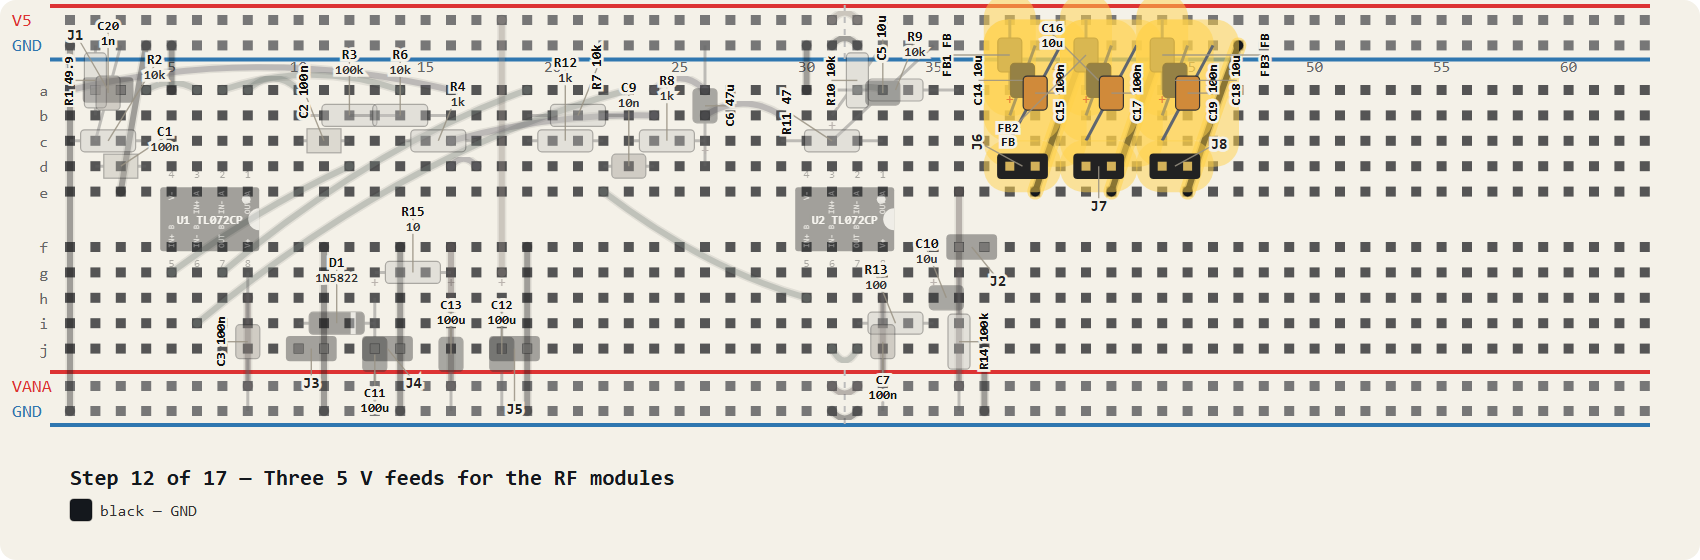
\includegraphics[width=\linewidth]{step-12.png}\end{center}
\vspace{-4pt}The ADF4351, the PA and the LNA each get a ferrite bead and their own 10 uF plus 100 nF pair, so one module's switching noise does not arrive at the next one along the rail. Identical blocks at columns 38, 41 and 44 — build one, check it, then repeat it twice.\par
{\footnotesize \begin{tabular}{P{0.12\linewidth}P{0.22\linewidth}P{0.56\linewidth}}
\toprule
\textbf{part} & \textbf{value} & \textbf{push it in at}\\
\midrule
FB1 & FB & 1→\textbf{TR+@38}, 2→\textbf{a38}\\
C14 & 10u & 1→\textbf{b38}, 2→\textbf{TR-@39}\\
C15 & 100n & 1→\textbf{c38}, 2→\textbf{TR-@40}\\
J6 & ADF4351 5V & 1→\textbf{d38}, 2→\textbf{d39}\\
FB2 & FB & 1→\textbf{TR+@41}, 2→\textbf{a41}\\
C16 & 10u & 1→\textbf{b41}, 2→\textbf{TR-@42}\\
C17 & 100n & 1→\textbf{c41}, 2→\textbf{TR-@43}\\
J7 & PA 5V & 1→\textbf{d41}, 2→\textbf{d42}\\
FB3 & FB & 1→\textbf{TR+@44}, 2→\textbf{a44}\\
C18 & 10u & 1→\textbf{b44}, 2→\textbf{TR-@45}\\
C19 & 100n & 1→\textbf{c44}, 2→\textbf{TR-@46}\\
J8 & LNA 5V & 1→\textbf{d44}, 2→\textbf{d45}\\
\bottomrule
\end{tabular}}\par
{\footnotesize \begin{tabular}{P{0.06\linewidth}P{0.12\linewidth}P{0.3\linewidth}P{0.42\linewidth}}
\toprule
\textbf{wire} & \textbf{colour} & \textbf{from → to} & \textbf{what it does}\\
\midrule
1 & black & \textbf{e39} → \textbf{TR-@41} & J6 GND\\
2 & black & \textbf{e42} → \textbf{TR-@44} & J7 GND\\
3 & black & \textbf{e45} → \textbf{TR-@47} & J8 GND\\
\bottomrule
\end{tabular}}\par
\checkline{5.00 V at all three of J6, J7, J8 with nothing plugged into them.}
\bbstep{13}{The ESP32 header and its series resistors}
\begin{center}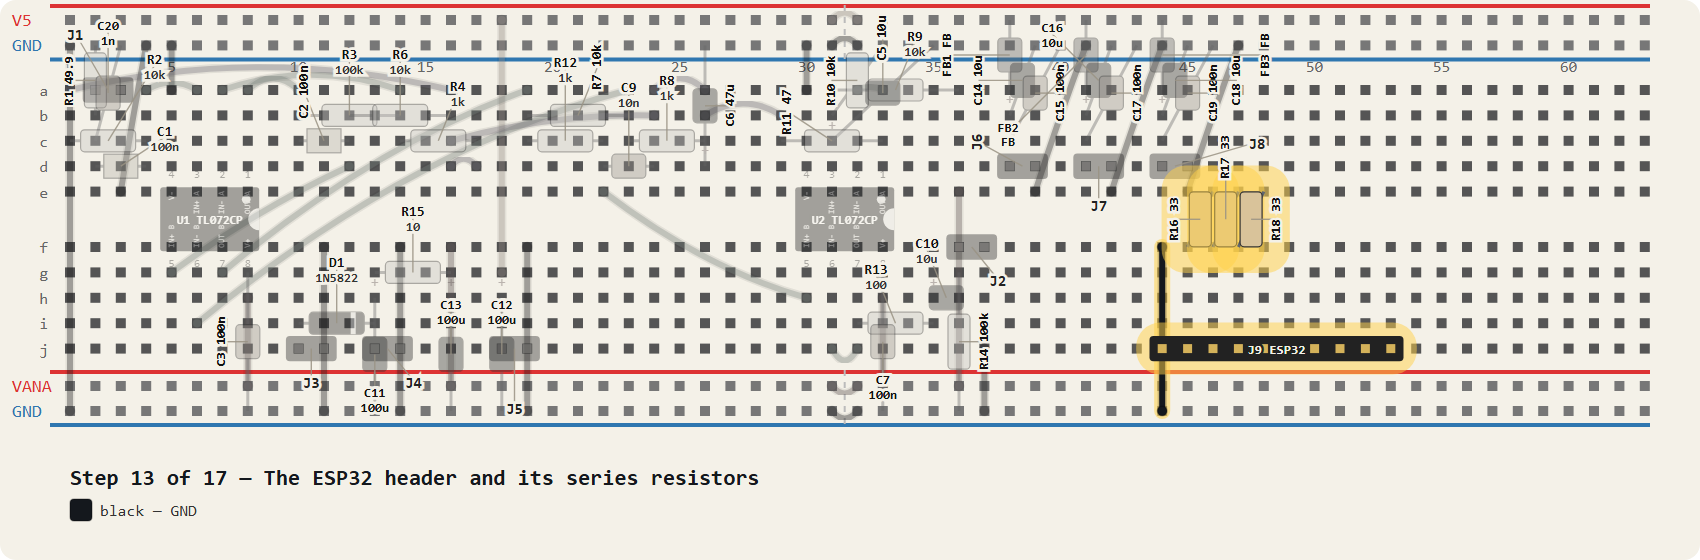
\includegraphics[width=\linewidth]{step-13.png}\end{center}
\vspace{-4pt}J9 is where the radar's ESP32 lands. R16 to R18 are 33 ohm series resistors on SCK, MOSI and LE: they damp the edges so a 2.54 mm breadboard run does not ring into the PLL's logic inputs. Each one hops the centre channel into the top bank.\par
{\footnotesize \begin{tabular}{P{0.12\linewidth}P{0.22\linewidth}P{0.56\linewidth}}
\toprule
\textbf{part} & \textbf{value} & \textbf{push it in at}\\
\midrule
J9 & ESP32 & 1→\textbf{j44}, 2→\textbf{j45}, 3→\textbf{j46}, 4→\textbf{j47}, 5→\textbf{j48}, 6→\textbf{j49}, 7→\textbf{j50}, 8→\textbf{j51}, 9→\textbf{j52}, 10→\textbf{j53}\\
R16 & 33 & 1→\textbf{f45}, 2→\textbf{e46}\\
R17 & 33 & 1→\textbf{f46}, 2→\textbf{e47}\\
R18 & 33 & 1→\textbf{f47}, 2→\textbf{e48}\\
\bottomrule
\end{tabular}}\par
{\footnotesize \begin{tabular}{P{0.06\linewidth}P{0.12\linewidth}P{0.3\linewidth}P{0.42\linewidth}}
\toprule
\textbf{wire} & \textbf{colour} & \textbf{from → to} & \textbf{what it does}\\
\midrule
1 & black & \textbf{f44} → \textbf{BR-@44} & J9 pin 1 GND\\
\bottomrule
\end{tabular}}\par
\checkline{Each resistor reads 33 ohms between its two strips, and nothing else.}
\bbstep{14}{SPI across to the ADF4351}
\begin{center}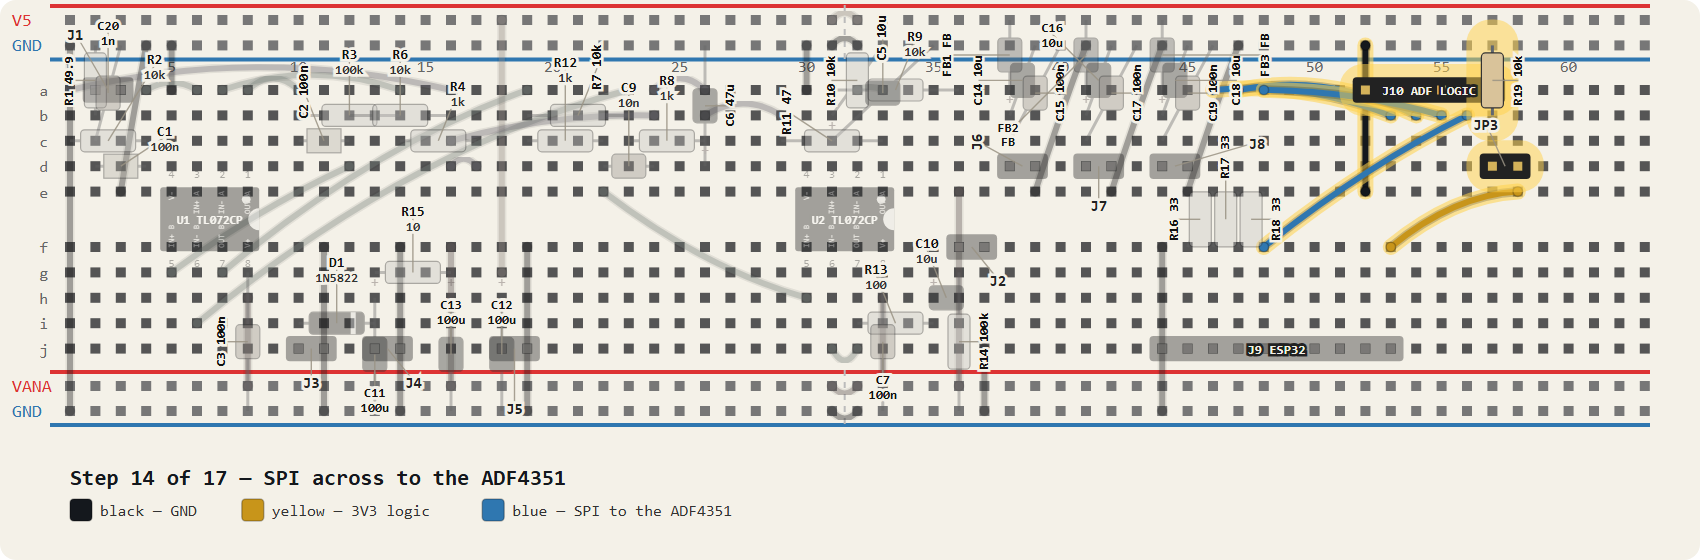
\includegraphics[width=\linewidth]{step-14.png}\end{center}
\vspace{-4pt}Four blue wires carry the damped SPI and the lock-detect line up to J10. R19 pulls CE down so the synthesiser's output stays OFF until something deliberately enables it, and JP3 is the link that enables it. The yellow wire brings 3V3 over from the ESP32 — the ADF4351 board is 3.3 V logic and needs no level shifting.\par
{\footnotesize \begin{tabular}{P{0.12\linewidth}P{0.22\linewidth}P{0.56\linewidth}}
\toprule
\textbf{part} & \textbf{value} & \textbf{push it in at}\\
\midrule
J10 & ADF LOGIC & 1→\textbf{a52}, 2→\textbf{a53}, 3→\textbf{a54}, 4→\textbf{a55}, 5→\textbf{a56}, 6→\textbf{a57}\\
R19 & 10k & 1→\textbf{b57}, 2→\textbf{TR-@57}\\
JP3 & CE EN & 1→\textbf{d57}, 2→\textbf{d58}\\
\bottomrule
\end{tabular}}\par
{\footnotesize \begin{tabular}{P{0.06\linewidth}P{0.12\linewidth}P{0.3\linewidth}P{0.42\linewidth}}
\toprule
\textbf{wire} & \textbf{colour} & \textbf{from → to} & \textbf{what it does}\\
\midrule
1 & black & \textbf{e52} → \textbf{TR-@52} & J10 pin 1 GND\\
2 & blue & \textbf{a46} → \textbf{b53} & R16 out (top col 46) -> J10 pin 2 SCK\_O (col 53)\\
3 & blue & \textbf{a47} → \textbf{b54} & R17 out (top col 47) -> J10 pin 3 MOSI\_O (col 54)\\
4 & blue & \textbf{a48} → \textbf{b55} & R18 out (top col 48) -> J10 pin 4 LE\_O (col 55)\\
5 & blue & \textbf{f48} → \textbf{b56} & J9 pin 5 LD (bottom col 48) -> J10 pin 5 LD (top col 56)\\
6 & yellow & \textbf{f53} → \textbf{e58} & J9 pin 10 3V3 (bottom col 53) -> JP3 pin 2 (top col 58)\\
\bottomrule
\end{tabular}}\par
\checkline{With JP3 off, CE reads 0 V. The radar must boot with RF off.}
\bbstep{15}{The A4988 stepper header}
\begin{center}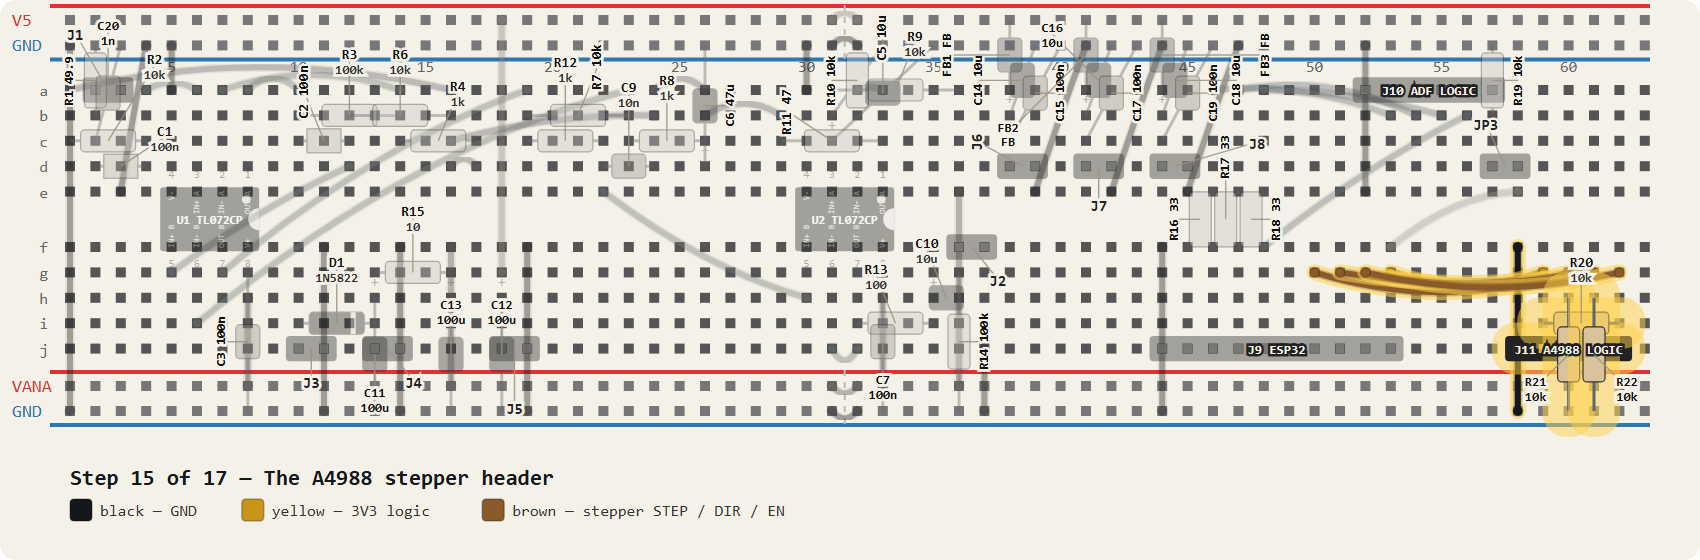
\includegraphics[width=\linewidth]{step-15.png}\end{center}
\vspace{-4pt}Only for the optional turntable; skip the whole step if you are not fitting one. R20 pulls EN up so the driver is disabled until the ESP32 says otherwise, and R21 and R22 pull STEP and DIR down so a floating input cannot make the motor twitch at power-up. The three brown wires are the control lines.\par
{\footnotesize \begin{tabular}{P{0.12\linewidth}P{0.22\linewidth}P{0.56\linewidth}}
\toprule
\textbf{part} & \textbf{value} & \textbf{push it in at}\\
\midrule
J11 & A4988 LOGIC & 1→\textbf{j58}, 2→\textbf{j59}, 3→\textbf{j60}, 4→\textbf{j61}, 5→\textbf{j62}\\
R20 & 10k & 1→\textbf{i59}, 2→\textbf{i62}\\
R21 & 10k & 1→\textbf{h60}, 2→\textbf{BR-@60}\\
R22 & 10k & 1→\textbf{h61}, 2→\textbf{BR-@61}\\
\bottomrule
\end{tabular}}\par
{\footnotesize \begin{tabular}{P{0.06\linewidth}P{0.12\linewidth}P{0.3\linewidth}P{0.42\linewidth}}
\toprule
\textbf{wire} & \textbf{colour} & \textbf{from → to} & \textbf{what it does}\\
\midrule
1 & black & \textbf{f58} → \textbf{BR-@58} & J11 pin 1 GND\\
2 & yellow & \textbf{g53} → \textbf{g59} & 3V3 -> J11 pin 2 / R20 (bottom col 59)\\
3 & brown & \textbf{g50} → \textbf{g60} & J9 pin 7 STEP (col 50) -> J11 pin 3 (col 60)\\
4 & brown & \textbf{g51} → \textbf{g61} & J9 pin 8 DIR (col 51) -> J11 pin 4 (col 61)\\
5 & brown & \textbf{g52} → \textbf{g62} & J9 pin 9 EN (col 52) -> J11 pin 5 (col 62)\\
\bottomrule
\end{tabular}}\par
\checkline{EN sits at 3V3, STEP and DIR at 0 V, with the ESP32 unplugged.}
\bbstep{16}{The SYNC divider back to the sound card}
\begin{center}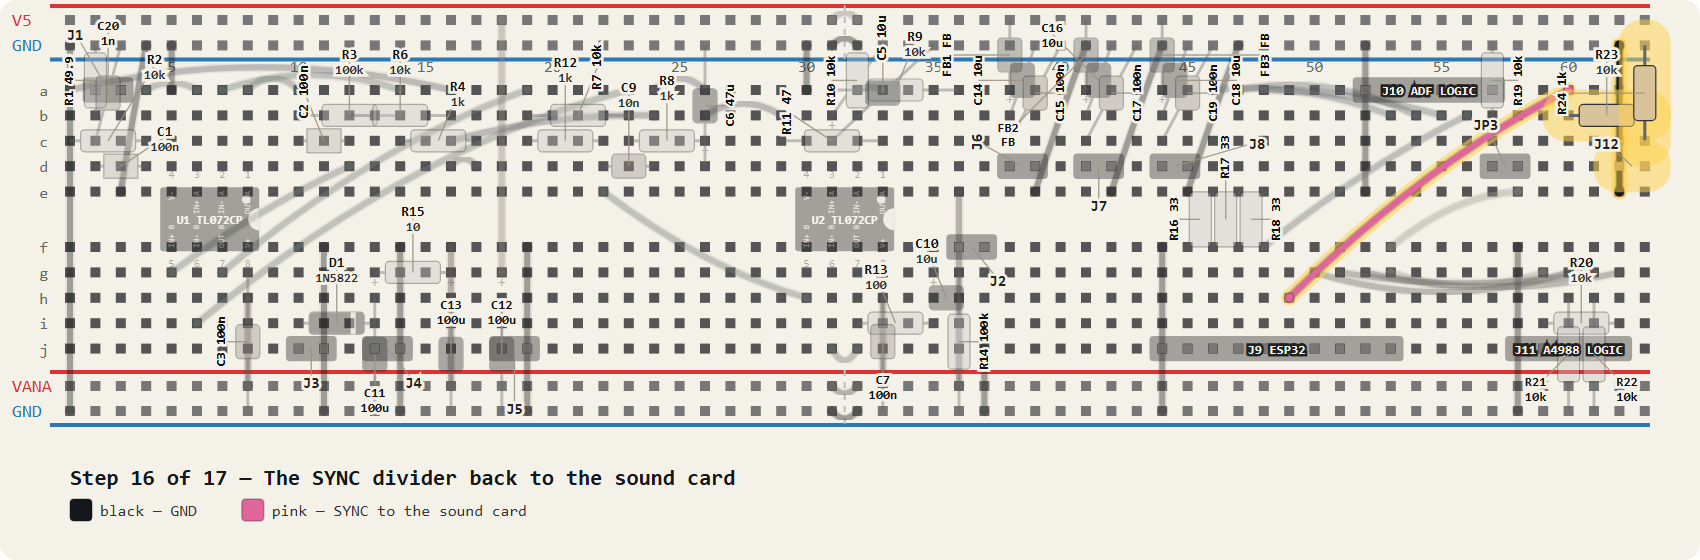
\includegraphics[width=\linewidth]{step-16.png}\end{center}
\vspace{-4pt}The last block, and the one that makes the whole radar measurable: R23 and R24 divide the ESP32's 3.3 V chirp marker down to about 0.3 V, which is a line-level signal the sound card's sync input (INPUT 2) can take. Without it the laptop cannot cut the beat signal into chirps and there is no range axis at all.\par
{\footnotesize \begin{tabular}{P{0.12\linewidth}P{0.22\linewidth}P{0.56\linewidth}}
\toprule
\textbf{part} & \textbf{value} & \textbf{push it in at}\\
\midrule
R23 & 10k & 1→\textbf{b60}, 2→\textbf{b63}\\
R24 & 1k & 1→\textbf{c63}, 2→\textbf{TR-@63}\\
J12 & AUDIO R & 1→\textbf{d63}, 2→\textbf{d62}\\
\bottomrule
\end{tabular}}\par
{\footnotesize \begin{tabular}{P{0.06\linewidth}P{0.12\linewidth}P{0.3\linewidth}P{0.42\linewidth}}
\toprule
\textbf{wire} & \textbf{colour} & \textbf{from → to} & \textbf{what it does}\\
\midrule
1 & black & \textbf{e62} → \textbf{TR-@62} & J12 GND\\
2 & pink & \textbf{h49} → \textbf{a60} & J9 pin 6 SYNC (bottom col 49) up to R23 (top col 60)\\
\bottomrule
\end{tabular}}\par
\checkline{A 135 Hz square wave of about 0.3 V at J12 once radar\_ctl is running.}
\bbstep{17}{Before you power anything}
\begin{center}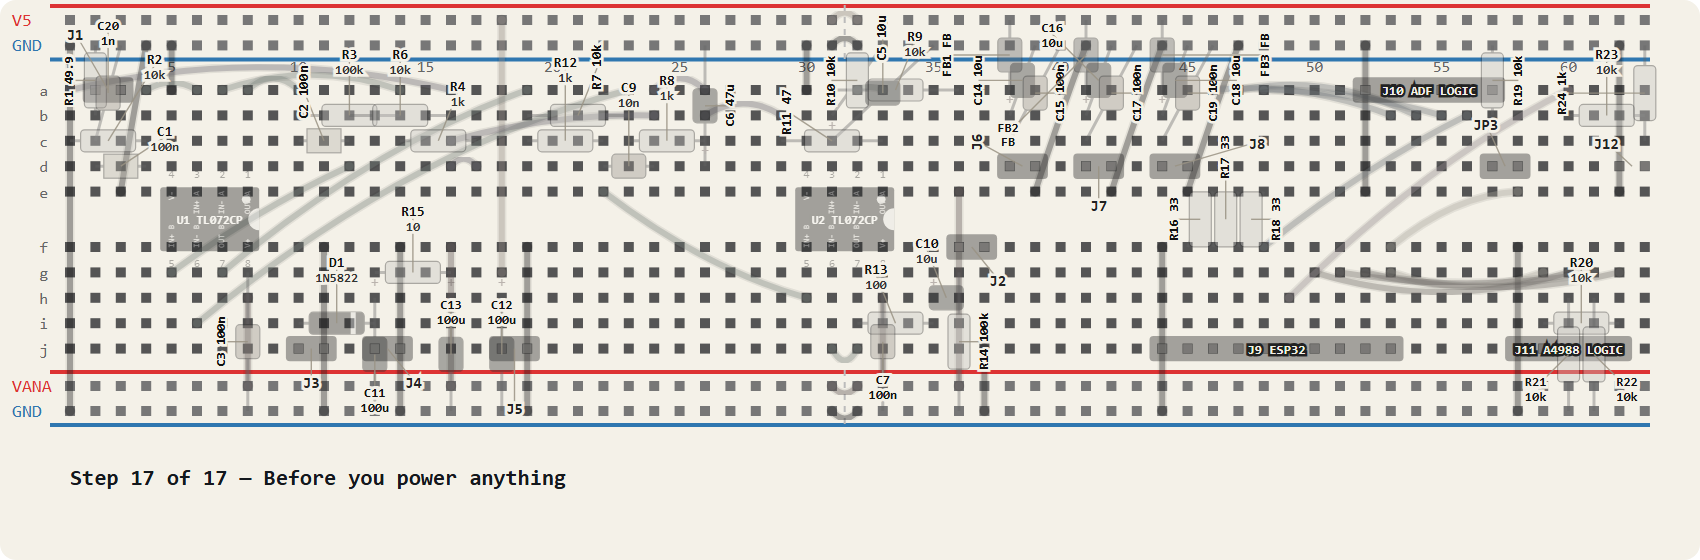
\includegraphics[width=\linewidth]{step-17.png}\end{center}
\vspace{-4pt}The board is finished. These are the measurements that catch a build error while it is still cheap, with the supply DISCONNECTED and nothing plugged into the headers.\par
\checkline{Ohm-meter, all with power off: GND to VANA, GND to V5 and GND to 3V3 must each read open (over 1 kohm). Any of them near zero is a short — find it before you connect 12 V. Then work the test blocks in breadboard/multisim/.}


\gate{step B17's resistance checks pass, with the 12\,V supply disconnected.}

\newpage
% ───────────────────────────────────────────────────────────── 5 power
\section{Stage 5: power}\label{sec:power}

\begin{warn}[Set the buck converter before it touches anything]
The LM2596 board arrives set to anything up to 12\,V out. Fed straight into the ADF4351 or an amplifier, that is an expensive few seconds. Set it to 5.00\,V first, with nothing on its output.
\end{warn}

\step{Set the buck converter to 5.00\,V}
\begin{enumerate}
  \item Wire J4 (pins 1 +, 2 −) to the buck's IN+ and IN−. Leave J5 and J6–J8 empty.
  \item Plug the 12\,V supply into J3. Put the meter on the buck's OUT+ and OUT−.
  \item Turn the small brass screw on the blue trimmer until the meter reads 5.00\,V. It is many turns end to end; be patient.
  \item Unplug the supply. Wire the buck's OUT+ and OUT− to J5.
\end{enumerate}

\step{Measure the rails}
Plug the 12\,V supply back in, with still nothing on J1, J2, J6–J12.

{\small
\begin{tabularx}{\linewidth}{@{}P{0.25\linewidth}P{0.25\linewidth}P{0.17\linewidth}L@{}}
\toprule
\textbf{rail} & \textbf{measure between} & \textbf{expect} & \textbf{if not} \\ \midrule
VPROT & D1 cathode (col 13) and GND & 11.6–11.8\,V & 0\,V: D1 backwards or the supply plug is wired backwards \\
VANA & bottom red rail and GND & 11.5–11.8\,V & low: R15 wrong value, or a short loading it \\
VREF & violet node (col 26) and GND & half of VANA, about 5.8\,V & 0 or VANA: R9/R10 or U2 pin 1/3 wiring \\
5\,V & top red rail and GND & 5.00\,V & re-set the buck \\
J6, J7, J8 & pin 1 to pin 2 & 5.00\,V each & 0\,V: ferrite bead not in the column \\
\bottomrule
\end{tabularx}}

\step{Connect the modules one at a time}
Supply off. Connect J6 to the ADF4351's 5\,V and GND pins, supply on, check it still reads 5\,V and the supply is not straining; supply off. Repeat with J7 to the PA and J8 to the LNA. Use red and black 22\,AWG twisted together, as short as reaches.

\gate{every rail in the table reads right, and all three modules powered together still leave 4.9–5.0\,V at their headers.}

\newpage
% ───────────────────────────────────────────────────────────── 6 firmware
\section{Stage 6: firmware and software}\label{sec:fw}

The firmware (\code{radar\_ctl}) and the laptop software (\code{ground\_station}) are in the repository's history rather than on this branch. Get a copy of both once:

\begin{note}[Getting the code]
\code{git archive 3f95c6d firmware ground\_station | tar -x -C \textasciitilde/radar-sw}\\[2pt]
That puts \code{firmware/radar\_ctl/radar\_ctl.ino} and the \code{ground\_station/} folder in \code{\textasciitilde/radar-sw}.
\end{note}

\step{Wire the ESP32 and the PLL's logic}
Only the logic, for now: no RF cables, PA and LNA unplugged.

{\small
\begin{tabularx}{\linewidth}{@{}P{0.16\linewidth}P{0.22\linewidth}P{0.22\linewidth}L@{}}
\toprule
\textbf{header} & \textbf{breadboard pin} & \textbf{goes to} & \textbf{note} \\ \midrule
J9 (10 wires) & 1 GND & ESP32 GND & \\
 & 2 SCK & ESP32 D18 & \\
 & 3 MOSI & ESP32 D23 & \\
 & 4 LE & ESP32 D5 & \\
 & 5 LD & ESP32 D19 & lock detect, back to the ESP32 \\
 & 6 SYNC & ESP32 D25 & \\
 & 7, 8, 9 & ESP32 D26, D27, D14 & STEP, DIR, EN: turntable only, may be left off \\
 & 10 3V3 & ESP32 3V3 & \\
J10 (6 wires) & 1 GND, 2 CLK, 3 DATA, 4 LE, 5 LD, 6 CE & ADF4351 header & match by the \textbf{printed names}, not by position: boards differ \\
JP3 & & a jumper cap & on = the PLL enabled \\
\bottomrule
\end{tabularx}}

\step{Flash radar\_ctl}
\begin{enumerate}
  \item In the Arduino IDE, install the \emph{esp32} board package (Espressif, 2.x or 3.x) and pick the board \textbf{“ESP32 Dev Module”}.
  \item Open \code{radar\_ctl.ino}. Check \code{F\_REF\_HZ} matches the crystal printed on your ADF4351 board's can: 25\,MHz on nearly all of them.
  \item Plug the ESP32 into the laptop by USB, pick its port, and upload. If the upload stalls at “Connecting…”, hold the BOOT button until it starts.
  \item Open the serial monitor at \textbf{115200} baud, line ending “Newline”, and type \code{?}.
\end{enumerate}

\checkline{the reply is a line of JSON ending in \code{"lock":1}, with \code{"rf":0} and \code{"sweep":0}. The board boots silent: it transmits nothing until you tell it to.}

{\small
\begin{tabularx}{\linewidth}{@{}P{0.3\linewidth}L@{}}
\toprule
\textbf{if you see} & \textbf{look at} \\ \midrule
nothing at all & baud rate 115200; the right port; a charge-only USB cable \\
\code{"lock":0} & \code{F\_REF\_HZ} against the crystal; CLK, DATA and LE swapped at J10; JP3 cap missing (CE low); 5\,V at J6 \\
\bottomrule
\end{tabularx}}

\step{Install the laptop software}
\begin{enumerate}
  \item In \code{ground\_station/}: \code{pip install -r requirements.txt} (Python 3.10 or newer).
  \item \code{python radar\_acquire.py --selftest}. It invents a target at 8\,m and should find it there. This proves the software before any hardware is involved.
  \item Plug in the UMC404HD and run \code{python -m sounddevice}. Note the number next to the UMC404HD's input: that is \code{--device N} from now on.
\end{enumerate}

\gate{\code{lock:1} on \code{?}, and the self-test finds its 8\,m target.}

\newpage
% ───────────────────────────────────────────────────────────── 7 mount and cable
\section{Stage 7: mount and cable}\label{sec:mount}

\begin{figure}[H]
\centering
\scalebox{0.92}{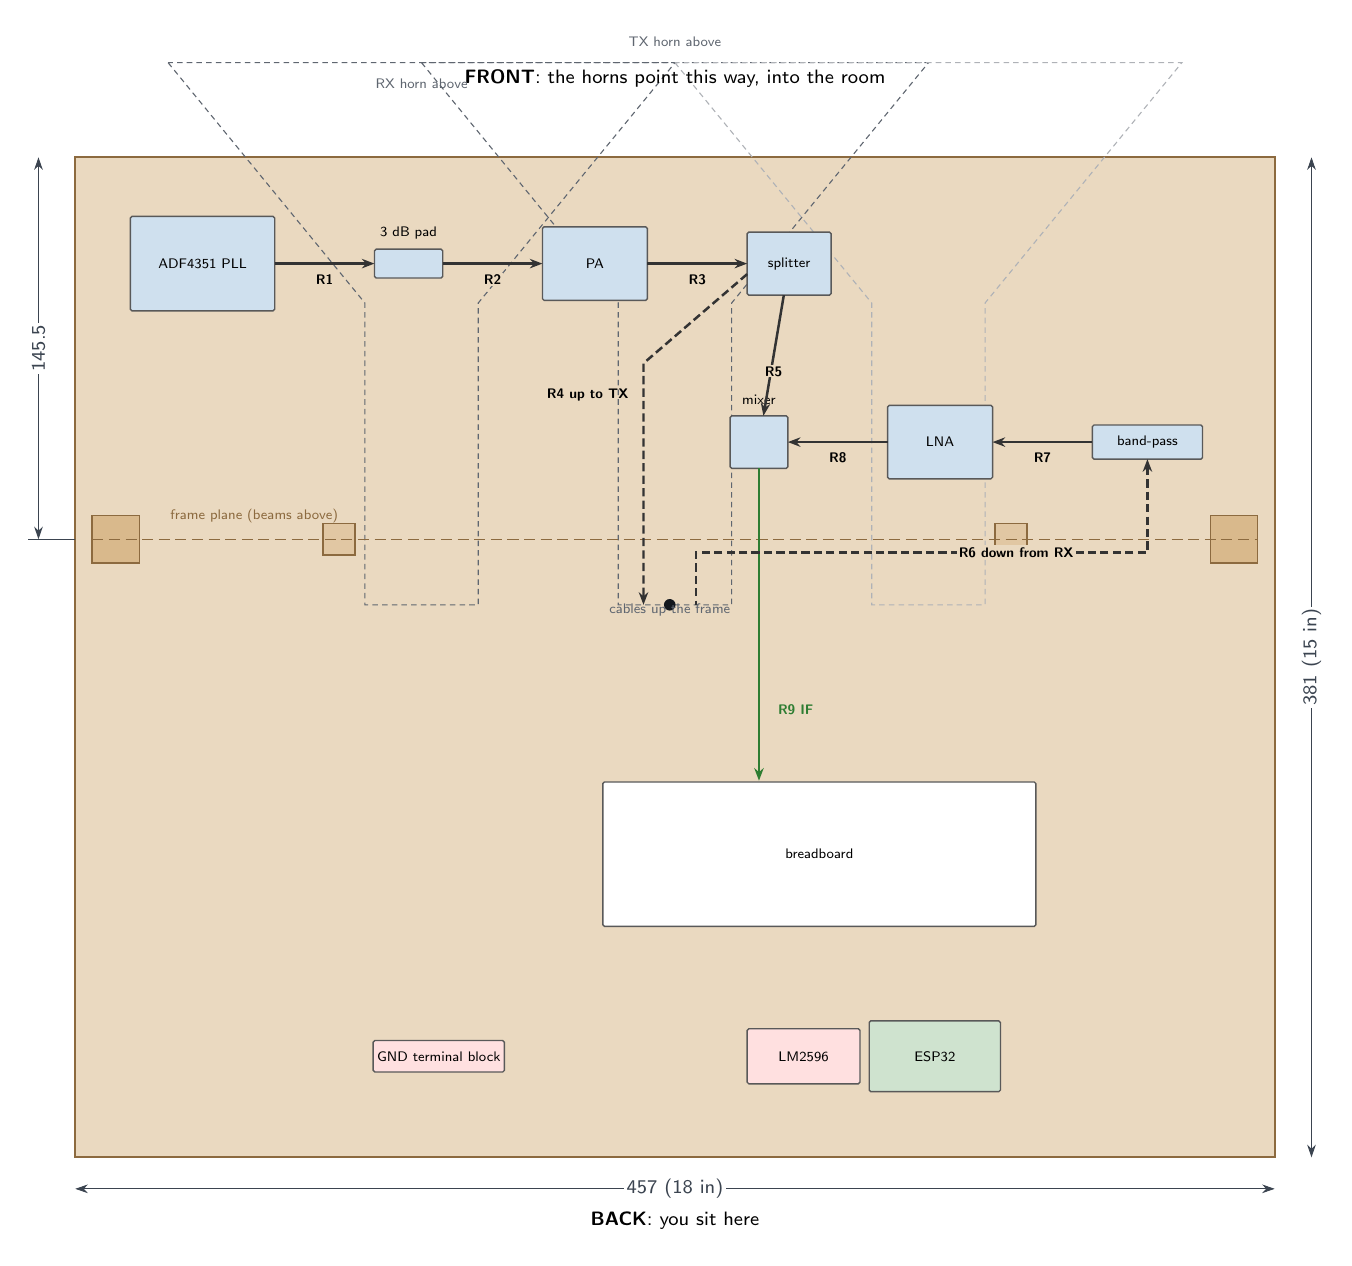
\begin{tikzpicture}[x=0.3333333333333333mm,y=0.3333333333333333mm,yscale=-1]
\path[woodpart,fill=wood!55] (-228.50,-190.50) rectangle (228.50,190.50);
\path[hidden] (-193.12,-226.55) -- (-118.15,-135.00) -- (-118.15,-20.00) -- (-74.95,-20.00) -- (-74.95,-135.00) -- (0.02,-226.55) -- cycle;
\path[hidden] (-96.57,-226.55) -- (-21.60,-135.00) -- (-21.60,-20.00) -- (21.60,-20.00) -- (21.60,-135.00) -- (96.57,-226.55) -- cycle;
\path[hidden,draw=muted!50] (-0.02,-226.55) -- (74.95,-135.00) -- (74.95,-20.00) -- (118.15,-20.00) -- (118.15,-135.00) -- (193.12,-226.55) -- cycle;
\node[font=\tiny,text=muted] at (-96.55,-218.55) {RX horn above};
\node[font=\tiny,text=muted] at (0.00,-234.55) {TX horn above};
\path[woodpart] (-222.00,-54.00) rectangle (-204.00,-36.00);
\path[woodpart,fill=wood!80] (-134.00,-51.00) rectangle (-122.00,-39.00);
\path[woodpart] (204.00,-54.00) rectangle (222.00,-36.00);
\path[woodpart,fill=wood!80] (122.00,-51.00) rectangle (134.00,-39.00);
\path[draw=woodedge,line width=0.4pt,dash pattern=on 4pt off 2pt] (-222.00,-45.00) -- (222.00,-45.00);
\node[font=\tiny,text=woodedge,anchor=west] at (-196.00,-54.00) {frame plane (beams above)};
\path[module,fill=rfmod] (-207.50,-168.00) rectangle (-152.50,-132.00);
\node[font=\tiny] at (-180.00,-150.00) {ADF4351 PLL};
\path[module,fill=rfmod] (-114.50,-155.50) rectangle (-88.50,-144.50);
\path[module,fill=rfmod] (-50.50,-164.00) rectangle (-10.50,-136.00);
\node[font=\tiny] at (-30.50,-150.00) {PA};
\path[module,fill=rfmod] (27.50,-162.00) rectangle (59.50,-138.00);
\node[font=\tiny] at (43.50,-150.00) {splitter};
\path[module,fill=rfmod] (159.00,-88.50) rectangle (201.00,-75.50);
\node[font=\tiny] at (180.00,-82.00) {band-pass};
\path[module,fill=rfmod] (81.00,-96.00) rectangle (121.00,-68.00);
\node[font=\tiny] at (101.00,-82.00) {LNA};
\path[module,fill=rfmod] (21.00,-92.00) rectangle (43.00,-72.00);
\path[module,fill=white] (-27.50,47.50) rectangle (137.50,102.50);
\node[font=\tiny] at (55.00,75.00) {breadboard};
\path[module,fill=pcb] (74.00,138.50) rectangle (124.00,165.50);
\node[font=\tiny] at (99.00,152.00) {ESP32};
\path[module,fill=red!12] (27.50,141.50) rectangle (70.50,162.50);
\node[font=\tiny] at (49.00,152.00) {LM2596};
\path[module,fill=red!12] (-115.00,146.00) rectangle (-65.00,158.00);
\node[font=\tiny] at (-90.00,152.00) {GND terminal block};
\node[font=\tiny] at (-101.50,-161.50) {3 dB pad};
\node[font=\tiny] at (32.00,-98.00) {mixer};
\path[draw=black!80,line width=0.9pt,-{Stealth[length=1.6mm]}] (-152.50,-150.00) -- (-114.50,-150.00);
\node[font=\tiny\bfseries,fill=wood!55,inner sep=0.5pt] at (-133.50,-144.00) {R1};
\path[draw=black!80,line width=0.9pt,-{Stealth[length=1.6mm]}] (-88.50,-150.00) -- (-50.50,-150.00);
\node[font=\tiny\bfseries,fill=wood!55,inner sep=0.5pt] at (-69.50,-144.00) {R2};
\path[draw=black!80,line width=0.9pt,-{Stealth[length=1.6mm]}] (-10.50,-150.00) -- (27.50,-150.00);
\node[font=\tiny\bfseries,fill=wood!55,inner sep=0.5pt] at (8.50,-144.00) {R3};
\path[draw=black!80,line width=0.9pt,-{Stealth[length=1.6mm]}] (41.47,-138.00) -- (33.69,-92.00);
\node[font=\tiny\bfseries,fill=wood!55,inner sep=0.5pt] at (37.58,-109.00) {R5};
\path[draw=black!80,line width=0.9pt,-{Stealth[length=1.6mm]}] (159.00,-82.00) -- (121.00,-82.00);
\node[font=\tiny\bfseries,fill=wood!55,inner sep=0.5pt] at (140.00,-76.00) {R7};
\path[draw=black!80,line width=0.9pt,-{Stealth[length=1.6mm]}] (81.00,-82.00) -- (43.00,-82.00);
\node[font=\tiny\bfseries,fill=wood!55,inner sep=0.5pt] at (62.00,-76.00) {R8};
\path[draw=sig,line width=0.9pt,-{Stealth[length=1.6mm]}] (32.00,-72.00) -- (32.00,47.00);
\node[font=\tiny\bfseries,text=sig] at (46.00,20.00) {R9 IF};
\path[draw=black!80,line width=0.9pt,dash pattern=on 3pt off 1.5pt,-{Stealth[length=1.6mm]}] (27.50,-146.00) -- (-12.00,-112.00) -- (-12.00,-20.00);
\node[font=\tiny\bfseries,anchor=east] at (-14.00,-100.00) {R4 up to TX};
\path[draw=black!80,line width=0.9pt,dash pattern=on 3pt off 1.5pt,{Stealth[length=1.6mm]}-] (180.00,-75.50) -- (180.00,-40.00) -- (8.00,-40.00) -- (8.00,-20.00);
\node[font=\tiny\bfseries,fill=wood!55,inner sep=0.8pt] at (130.00,-40.00) {R6 down from RX};
\fill[ink] (-2.00,-20.00) circle[radius=2.2];
\node[font=\tiny,text=muted,anchor=south] at (-2.00,-12.00) {cables up the frame};
\draw[dim] (-228.50,202.51) -- (228.50,202.51) node[dimlabel]{457 (18 in)};
\draw[dim] (242.51,-190.50) -- (242.51,190.50) node[dimlabel]{381 (15 in)};
\draw[dim] (-242.51,-190.50) -- (-242.51,-45.00) node[dimlabel]{145.5};
\path[ext] (-228.50,-45.00) -- (-246.50,-45.00);
\node[font=\scriptsize] at (0.00,-220.50) {\textbf{FRONT}: the horns point this way, into the room};
\node[font=\scriptsize] at (0.00,214.50) {\textbf{BACK}: you sit here};
\end{tikzpicture}
}
\caption{Where everything goes on the board, seen from above (from part 1). Horns at the top, your seat at the bottom.}
\end{figure}

\step{Mount the horns}
\begin{enumerate}
  \item Roll each horn onto its side so the connector points \textbf{left}. The pipe's narrow wall now sits on the saddle and the long side of the mouth runs up and down.
  \item Drop the pipe into its saddle and slide it until the saddle is \saddleBehind\ behind the throat (where flare meets pipe). Line the saddle cheeks with rubber or foam tape and tighten the two M4 clamp screws just until the horn will not slide.
  \item RX horn: the left saddle on the lower beam. TX horn: the saddle on the top beam. The right saddle on the lower beam stays empty for the second receiver.
  \item Lay a straightedge across the mouths: all three planes (RX, TX, and where the empty bay's mouth will be) should touch it. Adjust by sliding in the saddles.
\end{enumerate}
\checkline{RX horn centre \rxY\ above the board, \hornBase/2 = 96.6 left of the centre line; TX horn centre \txY\ above the board, on the centre line. The mouths overhang the board's front edge by about \overhang.}

\step{Lay out the modules}
Place the modules where the plan above puts them and fix them with foam tape or small brackets: the transmit chain (ADF4351, pad, PA, splitter) along the front, the receive chain (band-pass, LNA, mixer) behind it, the breadboard behind that. Keep the PA and LNA at least 10\,cm apart.

\step{The SMA cables}
Connect in this order, finger tight, then an eighth of a turn with the spanner. Look into each connector before mating it.

{\small
\begin{tabularx}{\linewidth}{@{}p{7mm}P{0.3\linewidth}P{0.3\linewidth}L@{}}
\toprule
\textbf{run} & \textbf{from} & \textbf{to} & \textbf{cable} \\ \midrule
R1 & ADF4351 RF OUT A & 3\,dB pad & 20\,cm \\
R2 & 3\,dB pad & PA in & 20\,cm (or pad straight on) \\
R3 & PA out & splitter input (S) & 20\,cm \\
R5 & splitter port 2 & mixer LO & 20\,cm \\
R7 & band-pass out & LNA in & 20\,cm \\
R8 & LNA out & mixer RF & 20\,cm \\
R4 & splitter port 1 & TX horn, up the middle of the frame & 1\,m, tied every 10\,cm \\
R6 & RX horn, down the middle of the frame & band-pass in & 60\,cm \\
R9 & mixer IF & breadboard J1: centre to pin 1, braid to pin 2 & pigtail \\
\bottomrule
\end{tabularx}}

\step{Audio and the last wires}
\begin{enumerate}
  \item J2 (beat) to the UMC404HD \textbf{INPUT 1}, J12 (sync) to \textbf{INPUT 2}, each with a shielded 1/4\,in TS cable: tip to pin 1, sleeve to pin 2.
  \item On the UMC404HD: 48\,V phantom power \textbf{off}; both gain knobs low (about 9 o'clock) to start; direct monitor irrelevant.
  \item In the laptop's sound settings: 44.1\,kHz, 16-bit, and every “enhancement”, automatic gain and noise suppression turned off.
\end{enumerate}
\begin{note}[Why sync goes on INPUT 2, not 3]
The stage-1 software records the interface's \emph{first two} inputs: beat, then sync. Plugged into INPUT 3, the sync is never read and the software reports no sync. When the second receiver goes in (stage 2), its beat takes INPUT 2 and the sync moves to INPUT 3, and the software is told to read three channels.
\end{note}

\gate{the whole chain is cabled and every SMA done up, and nothing is powered yet. A finger-tight SMA costs about 1\,dB, and you will chase it for an evening once there is a signal to blame it on.}

\newpage
% ───────────────────────────────────────────────────────────── 8 bring-up
\section{Stages 8 to 10: bring-up}\label{sec:bringup}

Power on in this order: 12\,V supply, then the ESP32's USB, then the UMC404HD's USB. Point the horns at an open room, not a wall a metre away.

\step{Checkpoint: the transmit power (if you can measure it)}
\code{CW 2440} parks the PLL on one frequency with RF on. With a power meter, or an RTL-SDR behind a 30\,dB attenuator, at the splitter's port 2 (the LO arm) in place of the mixer: \textbf{+10.5 ± 2\,dBm}. Type \code{RFOFF} and put the cable back. No meter? Skip this: the next check covers the same ground.

\step{First light: the leakage tone}
Type \code{SWEEP 1}. Open any audio recorder (Audacity is fine) on the UMC404HD and watch INPUT 1.

\checkline{a low tone with a strong part at about 26\,Hz. It is the transmitter leaking straight across the short gap into the receive horn, and it proves the PLL, the PA, the splitter, the LO, the LNA, the mixer and the amplifier all work, in one go. Set INPUT 1's gain so this tone peaks well below clipping, then never touch that knob again.}
\checkline{INPUT 2 shows a clean square wave at about 135\,Hz (6.4\,ms high, 1\,ms low), about 0.3\,V. That is the sync.}

\begin{note}[No leakage tone? Work backwards from the mixer]
Sync present but no tone: check LO drive first (R5 done up, splitter port 2), then the IF pigtail to J1, then the amplifier (each stage's output should sit at VREF with no signal). No sync either: \code{SWEEP 1} not sent, or J12's wire not at INPUT 2.
\end{note}

\step{First measurement: the walk test}
In \code{ground\_station/}, start the console and the acquisition (two terminals):

\code{python server.py}\\
\code{python radar\_acquire.py --device N --ctl /dev/ttyUSB0 --server http://localhost:8080}

(on Windows the port is \code{COM3} or similar). Open \code{http://localhost:8080}. Walk towards the horns from about 5\,m.

\checkline{range counts down as you approach and velocity reads negative, about your walking speed; walk away and it goes positive. Stand still and you vanish: that is not a fault, the radar subtracts everything that is not moving, along with the walls. Wave an arm and you come back.}

\gate{stand still at 3, 5 and 8\,m from the mouths, measured with a tape, while waving an arm: the printed range is within 0.4\,m each time.}

\step{The measurement that decides it: clutter cancellation}
Do this the day the chain first works. Point the radar at a still room with nobody moving. Record one block, then another a few seconds later, and subtract the range profiles. The ratio of the strongest echo to what is left is the clutter cancellation, in dB.

{\small
\begin{tabularx}{\linewidth}{@{}P{0.2\linewidth}L@{}}
\toprule
\textbf{you measure} & \textbf{what it means} \\ \midrule
over 50\,dB & the radar can find a small drone at 10\,m indoors: carry on \\
40–50\,dB & marginal at 10\,m, fine closer in \\
around 30\,dB & no amount of software will find the drone at 10\,m. The fix is mechanical: a rigid mount, more mass, no fan or air currents, nobody walking about \\
\bottomrule
\end{tabularx}}

\step{The drone link}
The drone's control link is on 915\,MHz so the radar can have the whole 2.4\,GHz band. Before the two are ever on together: with \code{SWEEP 1} running and the beam on the drone (props off), the link quality on the RadioMaster must stay at 100 and its signal strength must not move.

\gate{clutter cancellation over 50\,dB, and the drone link unaffected by the sweep. Then fly, keeping the drone moving towards or away at 0.1\,m/s or more: a pure hover is subtracted along with the walls.}

\newpage
% ───────────────────────────────────────────────────────────── 11 troubleshooting
\section{When something is wrong}\label{sec:trouble}

{\small
\begin{longtable}{@{}P{0.3\linewidth}P{0.66\linewidth}@{}}
\toprule
\textbf{symptom} & \textbf{likely cause, in order} \\ \midrule
\endhead
\code{"lock":0} & \code{F\_REF\_HZ} wrong; CLK/DATA/LE swapped at J10 (match the printed names); JP3 cap off; no 5\,V at J6 \\
no sync on INPUT 2 & \code{SWEEP} not on; J12 at the wrong input; R23/R24 not at columns 60 and 63 \\
sync present, no beat tone & LO cable R5; IF pigtail at J1 reversed; mixer RF/LO swapped; PA or LNA not powered \\
beat tone clips & INPUT 1 gain too high; or R4 is 1\,k while something upstream is too strong: fit 4.7\,k at R4 (gain 22) to diagnose \\
a steady hum, 50 or 60\,Hz & audio cables not shielded, or the laptop charger: try it on battery; star-ground everything at the terminal block \\
range reads consistently long or short & \code{--fs} not matching the sound card's real rate; a different sweep from the one the software assumes (use \code{--ctl} so it reads the sweep back) \\
a target at a fixed range that never moves & a reflection from the frame or the bench itself; check the foil screen is in place and nothing metal is near the mouths \\
nothing detected beyond a few metres & horns not facing the same way; RX cable R6 loose; the RX probe bent; clutter cancellation too low (stage 10) \\
the PA is very hot & normal is warm. Too hot to touch: check its supply is 5\,V, not 12 \\
\bottomrule
\end{longtable}}

\subsection*{Finished}
\begin{center}
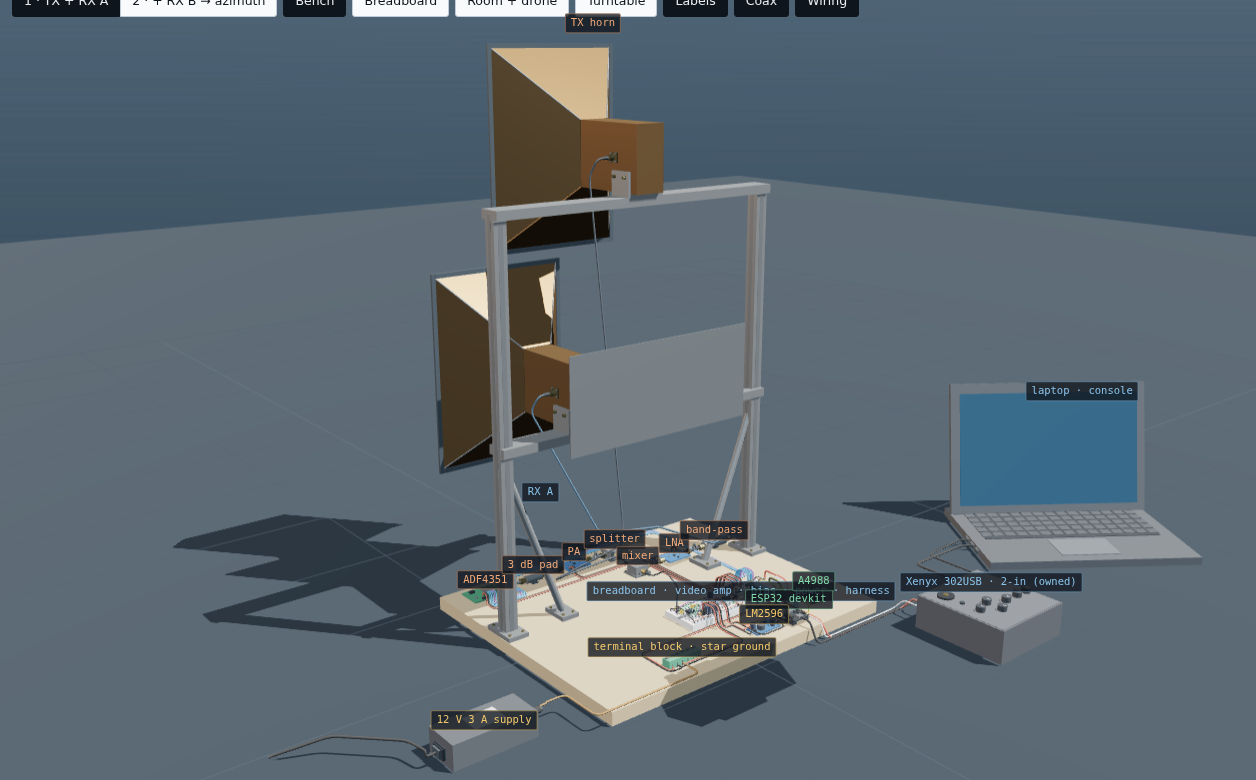
\includegraphics[width=0.9\linewidth]{bench_view.png}
\end{center}
That is the whole radar: range and radial speed of anything moving in the beam. The empty bay on the lower beam, the spare horn and the spare SPF5189Z are there for the second receiver, which adds direction.

\end{document}
